% \documentclass[conference, fleqn]{IEEEtran}
\documentclass[sigconf,draft]{acmart}

\usepackage{comment, color, graphicx, enumerate, amsmath, bm, mathtools, amssymb, subcaption, tikz, tabulary, url, algorithm, listings, algorithmicx, bbm, nth}
% \usepackage{subfig} % for subfloat
\usepackage[noend]{algpseudocode}
% \usepackage[export]{adjustbox}

\usepackage[inline]{trackchanges}
\addeditor{MA}
\newcommand\mehmet[1]{\add[MA]{#1}}

% \mehmet{I filled the following myself, does not mean it is correct!}
% \acmConference[SIGMETRICS]{ACM SIGMETRICS conference}{June 2017}{Urbana-Champaign, Illinois USA}
% \acmYear{2017}
% \copyrightyear{2017}

\begin{document}
% \newtheorem{theorem}{Theorem}

\title{Simplex Queues}
\maketitle
% #########################################  Abstract  ####################################### #
% \begin{abstract}
% \end{abstract}
% ##########################################  Intro  ######################################### #
\section{Introduction}
% LRC codes for storage
Locally repairable codes (LRC's) have been proposed to limit the number of nodes that need to be accessed to repair a systematic data symbol of a code \cite{rawat2014locality, tamo2014bounds}. Over the data encoded with LRC's, a data symbol can be recovered by accessing any one of the available disjoint repair groups where the number of repair groups for an arbitrary data symbol is called \emph{availability} of the code. Due to their availability, LRC codes are also named availability codes \cite{kadhe2015analyzing}. The number of nodes within each repair group is named as the \emph{locality} of the code. LRC's have been used for reliable data storage in distributed systems due to their low locality (repair bandwidth efficiency) and high availability (fault tolerance) \cite{huang2012erasure, primererasure, sathiamoorthy2013xoring, datta2013storage, li2013erasure, kuijper2014erasure}.
% \mehmet{May be worth to read "Erasure codes with simplex locality" again.}

% An example as in \cite{kadhe2015analyzing}, to explain LRC codes
For instance, suppose three data symbols $[a, b, c]$ are desired to be stored. A systematic LRC, namely \emph{simplex} code, encodes data into $[a, \: b, \: a+b, \: c, \: a+c, \: b+c, \: a+b+c]$. Assuming each encoded symbol is stored in a separate node, using the terminology in \cite{kadhe2015analyzing}, this scheme corresponds to the LRC(n=7, k=3, r=2, t=3) code where any data symbol can be downloaded by accessing either the systematic node or any of the $t=3$ disjoint repair groups of size $r=2$.

% What is this paper about?
While the availability of LRC's provide fault tolerance, it can also be possibly used to reduce data access time and increase throughput by simultaneously issuing download requests. Each download request for a data symbol can be served by the systematic node, repair group or groups depending on the availability of the code. Download time of distributed data that is encoded with LRC's is studied in \cite{kadhe2015analyzing}. Their results are for general LRC's and mostly for low download request arrival rate. In the case of high traffic of download requests, request get queued at the storage nodes, which makes the analysis of the download time intractable due to complex system dynamics governed by possibly many fork-join sub-systems in the system. This paper is inspired by the results presented in \cite{kadhe2015analyzing} and the results introduced on fork-join queueing systems in \cite{nelson1988approximate}. This paper focuses on analyzing data download time over data encoded using LRC's with locality two, i.e., each disjoint repair group for a data symbol consists of two nodes. Idea is to do the analysis for systems using LRC's with availability two by using the exact analysis of fork-join systems with two queues given in \cite{nelson1988approximate}. Main difference of this work than \cite{kadhe2015analyzing} is that we study the case where the download request arrival rate is high enough that requests may have to wait in the queue before getting served. As in \cite{kadhe2015analyzing}, analysis presented here is for downloading a data symbol (e.g., $a$) rather than downloading the whole data set (e.g., $[a,b,c]$).

% Our goal
Our goal is to understand the implications of using LRC codes to reliably store distributed data in terms of data access time. Our main methodology is to build good analytical models on the average data access time and use these models to argue about how storage systems perform under LRC's with different availability and different data access strategies. \mehmet{Should we define data access strategies before?}

% Our contribution?
As a start, we consider the \emph{split-to-all} access scheme where arriving request for downloading a data symbol is split to systematic node and all the repair groups. Starting with the simplest possible simplex code with availability one, we obtain close lower and upper bounds on the average download time. Then we argue that extending our findings for the simplest simplex code further to simplex codes with higher availability is hard. However, using ideas from queueing and renewal theory, we obtain relatively good lower and upper bounds on the average download time and observe that these bounds becomes almost exact for the simplest simplex code. Some observations on the gain achieved in access time by using codes with higher availability are given. Finally, another data access scheme \emph{split-to-one} where arriving request is forwarded to either the systematic node or one of the repair groups is considered and compared with the split-to-all scheme in terms of data access time and load balancing purposes.

% #######################################  System Model  ###################################### %
\section{System Model}
\label{sec:sec_sys_model}
\subsection{Encoding Model}
Data $[d_1, \ldots, d_k]$ to be stored consists of elements of a finite field. A systematic $(n,k)$ code is assumed to be used to generate coded symbols $[d_1, \ldots, d_k, c_1, \ldots, c_{n-k}]$, each of which is then stored is a separate node. We are interested in special class of LRC's for which each data symbol has locality $2$ and availability $t$. We name the resulting system as \emph{simplex queue} denote the it throughout as Simplex($t$) for $t \in Z^+$. \mehmet{Simplex(t) is a terminology we use here, but the code is not necessarily "simplex", not sure to keep it this way.} For instance, $(7,3)$ simplex code has locality $2$ and availability $3$ for each of the three data symbols and the system that employs it is denoted as Simplex($t=3$). We refer to a set of nodes that can repair a data symbol as the repair group of that symbol. \mehmet{Availability and locality are explained in Intro, I think no need to explain them again.} For example, Simplex($t=3$) code encodes data $[a, b, c]$ into $[a, \: b, \: a+b, \: c, \: a+c, \: b+c, \: a+b+c]$ where each code symbol is stored on nodes $1, \ldots, 7$. Each systematic data symbol can be recovered from three disjoint repair groups, e.g., besides the systematic node-$1$, $a$ can be recovered from \{node-$2$, node-$3$\}, \{node-$4$, node-$5$\}, \{node-$6$, node-$7$\}.

The simplex setup allows the download of a data symbol to be initiated in parallel by the systematic node and the disjoint repair groups. Code symbols downloaded from a repair group can then be used to recover the desired data symbol. We assume throughout the paper that the decoding procedure takes negligible time compared to the download time.

\subsection{Access Model}
We are interested in analyzing how the availability provided by the simplex setup affects the download time of individual data symbols. Each server (node) can serve only one download request at a time and the arriving requests get enqueued locally. Download of content at each server takes a random amount of time, which is referred to as \emph{service time}. We refer to a request for downloading a data symbol as a \emph{job} and the time that a job spends in the system between the arrival and the completion is referred to as the \emph{system time}.

We consider two different data access schemes. First type of system splits the arriving jobs to systematic server and all the repair groups, namely performing split-to-all. Job is finished once any one of these job replicas finish service. As soon as the first job replica finishes service, the remaining job replicas get canceled. Within each repair group there is a fork-join sub-system that forks the incoming job replica into sibling \emph{tasks}, which are then sent to two \emph{repair servers}. For the completion of a job replica in a repair group, both sibling tasks must finish service. Once the job completion is triggered by a repair group or systematic node, all the remaining job replicas and their sibling tasks get canceled. These redundant job replicas are expected to reduce the average time to access data. Second type of system forwards the arriving jobs to either the systematic node or any one of the repair groups, namely performing split-to-one. This load-balancing behavior trades access time with resource usage efficiency. Fig.~\ref{fig:fig_access_schemes} illustrates these access schemes.
\begin{figure}[hbt]
  \centering
  \begin{tikzpicture}
    \node at (0,2) {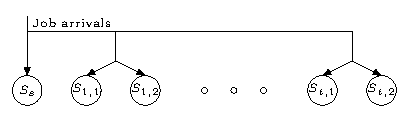
\includegraphics[scale=1]{fig_access_schemes_split_to_all}};
    \node at (0,0)  { 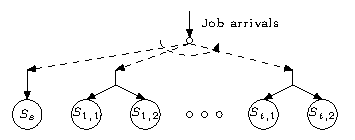
\includegraphics[scale=1]{fig_access_schemes_split_to_one}};
  \end{tikzpicture}
  \vspace*{-0.15cm}
  \caption{Data access models for simplex setup; (Top) split-to-all, (Bottom) split-to-one.}
  \label{fig:fig_access_schemes}
\end{figure}

We make the following assumptions throughout. Arriving tasks at the servers servers get serviced in order where tasks wait in a local queue. Service time at each server follows an independent exponential time. Jobs arrive according to a Poisson process of known rate.
\begin{comment}
% #########################################  Simplex  ######################################## %
\section{Problem Definition: Expected Hot Data Download Time for Simplex Queues}
\label{sec:sec_simplex_q}
To illustrate the complexity of the simplex queueing system, a possible system snapshot is given in Fig.~\ref{fig:fig_simplex_7_3}. 
\begin{figure}[hbt]
  \centering
  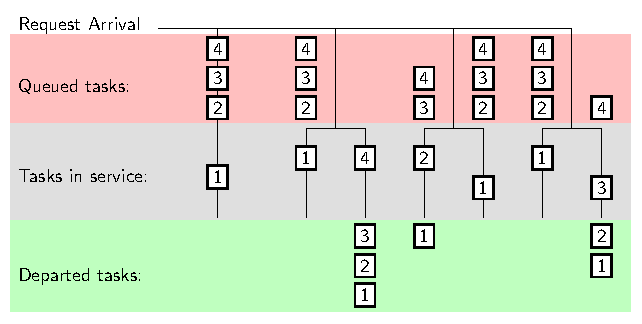
\includegraphics[scale=0.8]{Simplex73}
  \caption{System snapshot of a queue corresponding to the $(7, 3)$ simplex code i.e., Simplex($t=3$).}
  \label{fig:fig_simplex_7_3}
\end{figure}
%
This queueing system, namely the Simplex($t=3$), uses $(7, 3)$ binary simplex code. The complexity of system dynamics can be understood by observing that within a repair group fork-join queueing model is employed for downloading a data symbol. The state space of the system is complex since not only the number of tasks at each server but also the order and the jobs to which the tasks belong to must be identified by the state. Let $T$ be the random variable that denotes the time to download a symbol (i.e., job system time). Derivation of $E[T]$ for the low-traffic regime is presented in \cite{kadhe2015analyzing}. Using these results, under low traffic regime for Simplex($t=3$), one can find $E[T] = \frac{\beta(2, 0.5)}{2\mu} \approx \frac{0.46}{\mu}$. In \cite{kadhe2015analyzing}, an upper bound on $E[T]$ is found by using the more restrictive split-merge scheme. In this scheme, all the servers are blocked until the job is complete and thus multiple jobs cannot be in service simultaneously. The simulation results in \cite{kadhe2015analyzing} show that the upper bound suggested by SM model is loose unless the arrival rate is low.

Subsystems of simplex queues are fork-join queues with two servers (FJ-2) and an exact analysis of FJ queues is a hard problem. Steady-state behavior of such queues was analyzed in \cite{flatto1984two,flatto1985two}. An exact expression for the average system time for FJ-2 and a very good approximation for the general case with $n > 1$ servers are given in \cite{nelson1988approximate}.

\mehmet{Here we explain why we could not solve "mixed arrivals" and attempt to solve "all arrivals ask for the same symbol".} All the results presented in this paper consider the following system setup. Servers are just for fetching and streaming data to the user while the data is stored over a pool of shared resources. Thanks to this, we can fix some servers as the systematic servers while other servers as the repair server within the fixed repair groups. Therefore, all the arriving jobs can be treated the same even though they may possibly be for downloading different symbols. Even though this reduces the practicality of the system under consideration, it greatly simplifies the analysis of the system time by significantly reducing the state space complexity. Without this assumption, besides the arrival order, every task needs to be associated with a data symbol where for different data symbols different nodes must act as the systematic or repair servers. Another system level consideration which serves the same simplification is as follows. Suppose the coded symbols are both stored and served at the servers. However, only one symbol is frequently accessed over a time period while other symbols are rarely downloaded. This also allows us to focus on the case where job arrivals occur only for one symbol and so the systematic and repair servers can be fixed for all jobs. As an example for how this can be the case in practice, suppose the data symbols of interest are pieces of movies and web pages. During the day mostly web pages are expected to be requested while at night traffic for movies is expected to dominate.

% ######################################  Simplex(t=1)  ######################################## %
\section{Simplex queue with one repair group}
\label{subsec:subsec_simplex_t_1}
As the simplest version of the simplex queue introduced above, consider the setup with only one repair group, Simplex($t=1$) where a data symbol can be downloaded from either the systematic server or the repair group. Closely following the terminology in \cite{flatto1984two}, let the service rates at the systematic server and at two repair servers be $\gamma$, $\alpha$ and $\beta$ respectively. We refer to the systematic server as $S_s$ and servers in the repair group as $S_{1,1}$ and $S_{1,2}$. Let $\bm{N}(t) = [N_s(t), N_{1,1}(t), N_{1,2}(t)]$ be the system state where $N_{*}(t)$ is the number of tasks waiting or in-service in $S_*$ and denote $Pr\{\bm{N}(t) = [k, i, j]\}$ with $p_{k,i,j}(t)$. $\bm{N}(t)$ is a Markov process where the state space consists of tuples $(k, i, j), k, i, j \geq 0$. Job arrival process is assumed to be Poisson with arrival rate $\lambda$ ($Poisson(\lambda)$). Suppose that the stability is imposed and $lim_{t \rightarrow \infty} p_{k,i,j}(t) = p_{k, i, j}$. Balance equations for $\bm{N}(t)$ are
\begin{equation}
\label{eq:eq_simplest_simplex_balance}
  \begin{split}
    [\gamma & \mathbbm{1}(k \geq 1) + \alpha \mathbbm{1}(i \geq 1) + \beta \mathbbm{1}(j \geq 1)]p_{k,i,j} = \\
      & \lambda \mathbbm{1}(k \geq 1, i \geq 1, j \geq 1)p_{k-1,i-1,j-1} + \\
      & \gamma p_{k+1,i+1,j+1} + (\gamma + \alpha)p_{k+1,i+1,j} + (\gamma + \beta)p_{k+1,i,j+1}.
  \end{split}
\end{equation}
where $k, i, j \geq 0$ and $\mathbbm{1}$ is the indicator function.
For the exact analysis of the steady state behavior, computing the generating function $P_{w,x,y} = \sum p_{k,i,j}w^k x^i y^j$ from the balance equations given above for the steady state probabilities is formidable. Our approach is to look into approximating and/or obtaining close upper and lower bounds on the average system time $E[T]$.

% Even though data is coded and distributed over the servers differently for the MDS and Simplex setups, analysis of the job completion time for these two setups has similarities. Keeping arrival and service rates the same, the results for the MDS setup $E[T_{n=3,k=2}]$ gives an upper bound and $E[T_{n=3,k=1}]$ gives a loose lower bound on $E[T]$ for the Simplex setup as shown in Fig.~\ref{fig:fig_simplest_simplex_sim_up_low_bound}.
% \begin{figure}[h]
%   \centering
%   \includegraphics[width=0.5\textwidth, keepaspectratio=true]{fig_simplest_simplex_sim_up_low_bound.png}
%   \caption{Simulation results for $E[T_{n=3,k=2}]$, $E[T]$ and $E[T_{n=3,k=1}]$.}
%   \label{fig:fig_simplest_simplex_sim_up_low_bound}
% \end{figure}

% Explains modeling Simplex as M/G/1
In Simplex($t=1$), for every job, either all of the three tasks or only two of them (at $S_s$, $S_{1,1}$ or $S_s$, $S_{1,2}$) start service simultaneously, which we will refer to as the job starting setup. We call the former job starting setup where all the tasks start service at the same time as \emph{complete-start} while the latter one as \emph{partial-start}. Fig.~\ref{fig:fig_simplest_simplex_start_setup} shows an example where all the tasks of job $1$ starts service simultaneously while one of the task of job $2$ departs earlier than its siblings and the rest of the tasks will start service simultaneously upon the completion of job $1$. Overall, we define the job starting time as the time at which its last task starts service. According to this definition, multiple jobs cannot be in service simultaneously. For example in Simplex($t=1$), while a job is in service, at most a single task of the next job can be in service. Therefore, the simplex setup can be modeled as an M/G/1 queue where the arrivals represent jobs and departures represent job completions. The Pollaczek-Khinchin (PK) formula gives the expected response time:
\begin{equation}
  \label{eq:eq_simplex_t_1_PK}
  E[T] = E[V] + \frac{\lambda E[V^2]}{2(1 - \lambda E[V])}
\end{equation}
which requires the knowledge of the service time moments $E[V]$ and $E[V^2]$.
\begin{figure*}[hbt]
  \begin{center}
    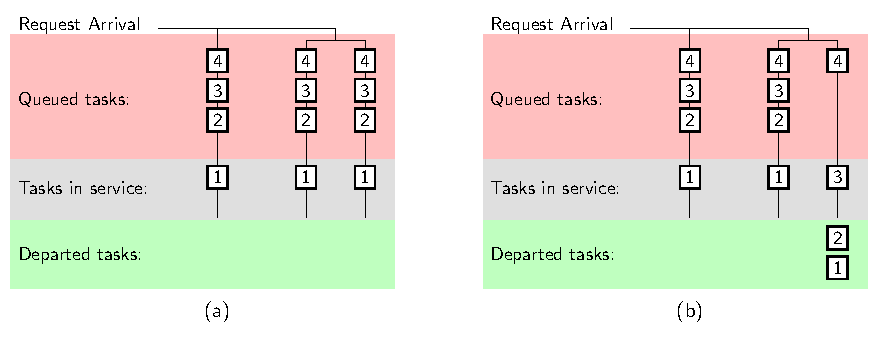
\includegraphics{Simplex32}
  \end{center}
  \vspace*{-0.5cm}
  \caption{Representation of (a) complete-start for job-$1$ and (b) partial-start for job-$2$ upon the completion of job-$1$ in Simplex($t=1$).\label{fig:fig_simplest_simplex_start_setup}}
\end{figure*}

Imagine that the synchronization between the tasks of every job is handled by a join queue, which is at the tail of the system queueing the departures from the servers. Join queue merges the incoming tasks based on their job id. Since the task coming from $S_s$ signals the job termination immediately, jobs waiting for synchronization must be started by the first task coming from either $S_{1,1}$ or $S_{1,2}$. Labeling each waiting job with the id $*$ of its initiator server, system state can be defined as the pair $\bm{n}(t) = (n_{1,1}(t), n_{1,2}(t))$ where $n_*$ denotes the number of jobs in the join queue with label $*$. Observe that $n_{1,1}(t)n_{1,2}(t) = 0$ must hold for all $t$ since the order of the tasks in $S_{1,1}$ and $S_{1,2}$ are preserved and receiving the tasks of the same job from both queues signals the job termination. Together with the number of jobs $N(t)$ at time $t$ waiting or in service in the system; $(N(t),\bm{n}(t))$ defines a Markov process for the overall system as shown in Fig.~\ref{fig:fig_simplex_t_1_mp__high_traff_aprox}. 
% \begin{figure}[htb]
%   \centering
% %     \node[anchor=west] at (0,0) {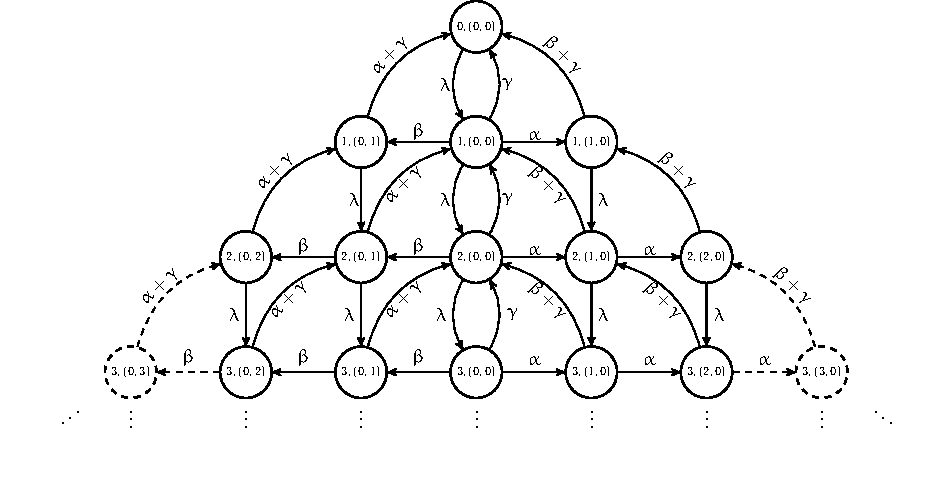
\includegraphics[scale=0.75, left]{MClongerpyramid}};
%   \begin{tikzpicture}
%     \node at (0,3) {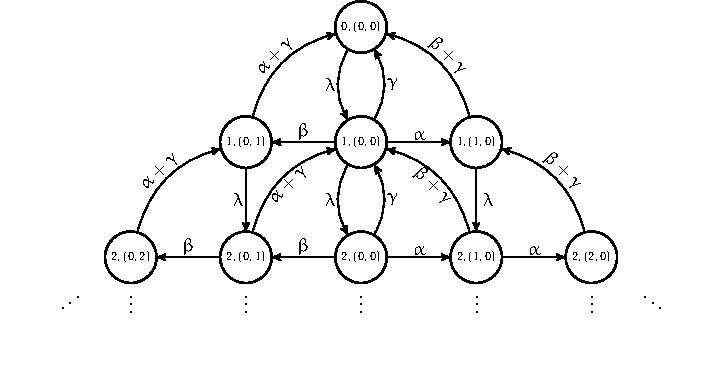
\includegraphics[scale=0.75]{MCpyramid}};
%     \node at (0,0)  { 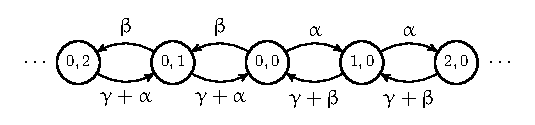
\includegraphics[scale=0.75]{S21JoinHighT}};
%   \end{tikzpicture}
%   \vspace*{-0.5cm}
%   \caption{Markov process (Top) for Simplex($t=1)$, and (Bottom) its high traffic approximation.}
%   \label{fig:fig_simplex_t_1_mp__high_traff_aprox}
% \end{figure}

% Here we conclude by outlining our ideas to find a closed-form solution for the average system for Simplex($t=1$). First we try to get better understanding of the service time by using complete and partial-start concepts introduced above. Finding an expression for the service time requires computing limiting fraction of jobs that make complete and partial-start and this requires solving the MC on the left in Fig. \ref{fig:fig_simplex_t_1_mp__high_traff_aprox}, which can be proven to be tedious by showing an approximate-analytical and exact-numeric solution. Therefore, our idea is to use high-traffic approximation of this MC, which yields a single-dimensional chain that is easy to analyze as shown on the right in Fig. \ref{fig:fig_simplex_t_1_mp__high_traff_aprox}. Finally first and second moments for the service time can be computed under the high-traffic assumption which then by plugging into PK formula would give a close lower bound on the actual average system time.

The job service time follows a general distribution. Defining random variable $J$ as the starting setup of the job with values $c$ and $p$ denoting complete-start and partial-start. Therefore, we can write the service time distribution for an arbitrary job as $Pr\{V \geq v\} = f_J(c)Pr\{V_c \geq v\} + f_J(p)Pr\{V_p \geq v\}$ where $Pr\{V_c \geq v\} = Pr\{V \geq v | J=c\}$ and $Pr\{V_p \geq v\} = Pr\{V \geq v | J=p\}$ denote the service time distributions given a job makes a complete or partial-start respectively. Random variables $V$, $V_c$ and $V_p$ are non-negative and using $E[V] = \int_{0}^{\infty} Pr\{V \geq v\}ds$ and $E[S^2] = \int_{0}^{\infty} 2sPr\{V \geq v\}ds$, the first and second moments of the general service time distribution can be computed as follows:
\begin{equation}
  \label{eq:eq_simplest_simplex_serv_time_moments}
  \begin{split}
    & E[V] = f_J(c)E[V_c] + f_J(p)E[V_p] \\
    & E[V^2] = f_J(c)E[V_c^2] + f_J(p)E[V_p^2]
  \end{split}
\end{equation}
In partial-start, one task starts service at $S_s$ simultaneously with the other one starting service at either $S_{1,1}$ or $S_{1,2}$. For simplicity, consider $\alpha = \beta = \mu$. Completion of either of these tasks signal the job termination; $V_p = min\{Exp(\gamma), Exp(\mu)\}$, so $V_p$ is $Exp(\gamma+\mu)$. In complete-start, tasks start service simultaneously at all servers, so $V_c = min\{Exp(\gamma), max\{Exp(\mu), Exp(\mu)\}\}$, then one can find $E[V_c] = 2/(\gamma+\mu)-1/(\gamma+2\mu)$ and $E[V_c^2]=4/(\gamma+\mu)^2-2/(\gamma+2\mu)^2$. In a split-merge setup, every job makes a complete-start, which is studied in \cite{kadhe2015analyzing}, so $E[V_c] = 0.5\mu^{-1}\beta(2,0.5) = 0.665\mu^{-1}$ and $E[V_c^2] = 7/9\mu^{-2}$. Note that here, average system time decreases as more jobs make a partial-start since $E[V_p] < E[V_c]$ and $E[V_p^2] < E[V_c^2]$. What is left missing are the values for $f_J(p)$ and $f_J(c)$. One can write:

% When the simplex setup is in stable working condition, process shown in Fig.~\ref{fig:fig_simplex_t_1_mp__high_traff_aprox} is ergodic. Starting setup $J_i$ of job $i$ depends on the state of the system $\bm{N}(a_i)$ found when job arrives at time $a_i$. Since Poisson arrivals see time averages \cite{wolff1982poisson}, $\lim_{i \rightarrow \infty} f_{\bm{N}(a_i)}(\bm{s}) = p_{\bm{s}}$ where $p_{\bm{s}}$ is the steady-state probability of system being in state $\bm{s}$, we can see that $\lim_{i \rightarrow \infty} J_i = J$ as
\begin{equation*}
  \begin{split}
    f_{J_i}(j) &= \sum_{\bm{s}} f_{J_i,\bm{N}(a_i)}(j | \bm{s})f_{\bm{N}(a_i)}(\bm{s}), \\
    \lim_{i \rightarrow \infty} f_{J_i}(j) &= \sum_{\bm{s}} f_{J,\bm{N}(a)}(j | \bm{s}) p_{\bm{s}} = f_J(j).
  \end{split}
\end{equation*}
where density functions are shown with $f$. Next we will argue about computing job starting setup distribution $f_J(j)$. Sub-sequence of the job arrivals that see an empty system forms a renewal process (Theorem 5.5.8 in \cite{gallager2013stochastic}) and we define $R_j(t) = \mathbbm{1}\{J(t) = c\}$ as a renewal-reward function where ${J(t) = c}$ is the event that job in service at time $t$ made a complete-start and $\mathbbm{1}$ is the indicator function of the event. Limiting time and ensemble average of $R_j(t)$ will be the same (Theorem 5.6.2 in \cite{gallager2013stochastic}), and since $R_j(t)$ is a binary-valued function, its limiting ensemble average will give the limiting probability of an arbitrary job to make a complete-start, as written below:
\begin{equation*}
  \begin{split}
    f_J(c) &= 
      \lim_{\tau \rightarrow \infty} E[R_j(\tau)] =
      \lim_{\tau \rightarrow \infty} Pr\{R_j(\tau) = 1\} \\
    &= \lim_{\tau \rightarrow \infty} \frac{1}{\tau} \int_{-\infty}^{\tau}R_j(\tau) = \frac{E[R_n]}{E[X]}
  \end{split}
\end{equation*}
where $R_n = \int_{S_{n-1}^r}^{S_n^r}R_j(t)dt$, $S_{n-1}^r$ and $S_n^r$ are the $(n-1)$th and $n$th renewal epochs (i.e., epochs for job arrivals that find the system empty), and $X$ is the iid inter-renewal interval. To compute $f_J(c)$, we need $E[R_n]$ and $E[X]$, which are hard to find. Also the Markov process shown in Fig.~\ref{fig:fig_simplex_t_1_mp__high_traff_aprox} is tedious to analyze (see Appendix \ref{subsec:subsec_simplex_t_1_pyramid_mp_analysis}). That is why we try to estimate $f_J(c)$ by studying a different system approximating the actual setup.

% ---------------------------------  High-traffic assumption  ----------------------------- %
\subsection{Analysis under high-traffic regime}
\label{subsec:subsec_simplex_t_1_analysis_w_high_traff}
Suppose $\lambda$ is very close to its critical value for stability and the system is started at $-\infty$. Starting to observe the system state at $t = 0$, we assume that queues $S_s$, $S_{1,1}$ and $S_{1,2}$ are never empty, which is a rather crude assumption and holds only when system is unstable. We will refer to this set of working conditions as "high-traffic regime''. Using the assumption that queues are never empty, state of the join queue $\bm{n}(t)$ itself is a simple Markov process shown on the bottom in Fig.~\ref{fig:fig_simplex_t_1_mp__high_traff_aprox}. Note that after every transition, an exponential service time is restarted for each server and the first task completion causes the process to transit to another state. Here task cancellation at a server due to job completion is not considered as a task completion. Comparing the two Markov processes in Fig.~\ref{fig:fig_simplex_t_1_mp__high_traff_aprox}, one can see that process for the high traffic regime can be obtained from the other one as follows: (1) Introduce additional transitions of rate $\alpha$ from state $(i,(i,0))$ to $(i+1,(i+1,0))$ and transitions of rate $\beta$ from state $(i,(0,i))$ to $(i+1,(0,i+1))$ for $i \geq 0$, (2) Gather all the states $(i,(m,n))$ for all $i \geq 0$ into a "super state", (3) Observe that process represented with these super-states is the same as the process for high-traffic regime. Thus, average system time under high-traffic regime will be always less than the average system time experienced by a job under stable working conditions because high-traffic regime has the effect of placing extra state transitions that enables the system to serve jobs faster. We will elaborate on this more later in this section. Steady-state balance equations for the process under high-traffic regime is shown in \eqref{eq:eq_simplest_simplex_join_balance_high_traffic}.
\begin{equation}
\label{eq:eq_simplest_simplex_join_balance_high_traffic}
  \alpha p_{i,0} = (\gamma + \beta) p_{i+1,0}\quad\text{and}\quad
   \beta p_{0,i} = (\gamma + \alpha) p_{0,i+1}, ~i \geq 0.
\end{equation}
where $lim_{t \rightarrow \infty} Pr\{\bm{n}(t) = [i,j]\} = p_{i,j}$. Solving balance equations:
% \begin{align*}
%   p_{i,0} = (\frac{\alpha}{\beta + \gamma})^i p_{0,0}, i \in [1, \infty) \\
%   p_{0,i} = (\frac{\beta}{\alpha + \gamma})^i p_{0,0}, i \in [1, \infty)
% \end{align*}
\begin{equation}
\label{eq:eq_simplest_simplex_steady_state}
p_{i,0} = (\frac{\alpha}{\beta + \gamma})^i p_{0,0} \quad\text{and}\quad
   p_{0,i} = (\frac{\beta}{\alpha + \gamma})^i p_{0,0}, ~i \geq 1.
\end{equation}
by the axiom of probability,
$(1 + \sum_{i=1}^{\infty} (\frac{\beta}{\alpha + \gamma})^i + (\frac{\alpha}{\beta + \gamma})^i )p_{0,0} = 1$
assuming $\beta < \alpha + \gamma$ and $\alpha < \beta + \gamma$,
\[ p_{0,0} = (1 +  \frac{\beta}{\alpha + \gamma - \beta} + \frac{\alpha}{\beta + \gamma - \alpha} )^{-1} = \frac{\gamma^2-(\alpha-\beta)^2}{\gamma(\alpha+\beta+\gamma)} \] 
from which $p_{i,0}$ and $p_{0,i}$ can be computed. 
Other useful quantities are:
$$ \sum_{i=1}^\infty p_{i,0} = \frac{\alpha(\alpha+\gamma-\beta)}{\gamma(\alpha+\beta+\gamma)}, \quad\quad \sum_{i=1}^\infty p_{0,i} = \frac{\beta(\beta+\gamma-\alpha)}{\gamma(\alpha+\beta+\gamma)}$$
For tractable analysis, we will continue with the assumption $\alpha = \beta = \mu$, then we have $p_{0,0} = \frac{\gamma}{\gamma+2\mu}$ and $\sum_{i=1}^{\infty} p_{i,0} = \sum_{i=1}^{\infty} p_{0,i} = \frac{\mu}{\gamma+2\mu}$. Next, we will use these steady-state probabilities for the high-traffic regime to obtain some estimates and/or lower bounds for the quantities of interest.

% ---------------------------------  Winning frequencies  ----------------------------- %
\subsection{Winning frequencies}
\label{subsec:subsec_simplex_t_1_winning_freqs}
A job is completed upon the completion of the terminating task at one of the servers. Fraction of the jobs terminated by a server can be computed from the steady-state probabilities of the Markov chain (MC) that is embedded in the Markov process $\bm{n}(t)$ discussed above. As previously devised for Simplex($t=1$), the state at the join queue is $\bm{n}(t) = (n_{1,1}(t), n_{1,2}(t))$ where $n_*$ denotes the number of jobs with label $*$ waiting in the join queue. We see from  \eqref{eq:eq_simplest_simplex_join_balance_high_traffic} that transition rates out of every state are equal. Thus steady-state probabilities of the Markov process ($p_i$: limiting fraction of the time process spends in state $i$) and the embedded chain ($\pi_i$: limiting fraction of the state transitions into state $i$) are equal as can be seen below.
\[ \pi_i = \frac{p_i\nu_i}{\sum_i p_i\nu_i} = \frac{p_i\nu}{\nu\sum_i p_i} = p_i \text{ where } \nu_i = \nu = \gamma+2\mu \]

Let the fraction of the job terminations signaled by the servers $S_s$, $S_{1,1}$ and $S_{1,2}$ be $w_s$, $w_{1,1}$ and $w_{1,2}$ respectively. We define $w_*$ as the "winning frequency" of the server $*$ where a server wins if it signals the termination of a job. To find $w_*$, first we need to find the limiting fraction of state transitions which represent job terminations $f_s$, $f_{1,1}$, $f_{1,2}$ that are signaled by the respective servers $S_s$, $S_{1,1}$, $S_{1,2}$ in the embedded MC as follows:
\begin{align*}
  & f_s = \pi_{0,0}\frac{\gamma}{\nu} + \sum_{i=1}^{\infty} \pi_{i,0}\frac{\gamma}{\nu} + \sum_{i=1}^{\infty} \pi_{0,i}\frac{\gamma}{\nu} = \frac{\gamma}{\nu}, \\
  & f_{1,1} = \sum_{i=1}^{\infty} \pi_{0,i}\frac{\alpha}{\nu} = (\frac{\mu}{\nu})^2 \quad\text{and}\quad f_{1,2} = \sum_{i=1}^{\infty} \pi_{i,0}\frac{\beta}{\nu} = (\frac{\mu}{\nu})^2
\end{align*}
which then can be used to compute the winning frequencies as follows: denote the fraction of state transitions that represent job departures as $f_{jd} = f_s + f_{1,1} + f_{1,2} = \frac{\gamma\nu+2\mu^2}{\nu^2}$, so $w_s = f_s/f_{jd} = \frac{\gamma\nu}{\gamma\nu+2\mu^2}$, $w_{1,1} = f_{1,1}/f_{jd} = w_{1,2} = f_{1,2}/f_{jd} = \frac{\mu^2}{\gamma\nu+2\mu^2}$.

Winning frequencies reported in Fig.~\ref{fig:fig_simplest_simplex_sim_winning_freqs_avg} are obtained by simulating a system with $\gamma = \mu$. As the arrival rate increases simulated values converge to the values $w_s = 0.6$, $w_{1,1} = w_{1,2} = 0.2$ that are computed using the expressions that are found above. In high-traffic model, queues are never empty while under lower $\lambda$, fraction of the time repair servers spend idle is non-zero. This causes the repair group to win less number of times than it would under the higher traffic load. This is why expression we found for $w_s$ using high-traffic approximation gives a lower bound and expressions for $w_{1,1}$ and $w_{1,2}$ give upper bound.
\begin{figure}[h]
 \centering
 \includegraphics[width=0.5\textwidth, keepaspectratio=true]{fig_simplest_simplex_sim_winning_freqs_avg.png}
 \caption{Simulation results for winning frequencies of the servers in Simplex($t=1$).}
 \label{fig:fig_simplest_simplex_sim_winning_freqs_avg}
\end{figure}

% ---------------------------------  Average system time  ------------------------ %
\subsection{Average system time}
\label{subsec:subsec_simplex_t_1_avg_sys_time}
Under high-traffic regime, there is always a job in the queue waiting to receive service. Let a new job start at time $\tau$ upon the departure of the previous job at $\tau^-$, the starting setup of the job is determined by the state of the join queue $\bm{n(\tau^-)}$. Note that $\bm{n(\tau^-)}$ is the state after the last departing job arrives at the join queue. Therefore, $\bm{n(\tau^-)}$ is determined by the last state transition at the join queue that is triggered by a job departure. In other words, every transition in the Markov chain embedded in $\bm{n(t)}$ that is triggered by a departing job defines the starting setup of the subsequent job. Therefore, we can find the limiting fraction of the jobs that make partial ($f_{jp}$) or complete-start ($f_{jc}$) by following the approach we used in Subsection \ref{subsec:subsec_simplex_t_1_winning_freqs}.

In Subsection \ref{subsec:subsec_simplex_t_1_winning_freqs}, we defined $f_{jd}$ as the fraction of state transitions corresponding to job departures and here we also define $f_c$ as the fraction of state transitions into a complete-start for the subsequent job. Then, the values of $f_{jp}$ and $f_{jc}$ can be calculated as
\begin{align*}
  & \begin{aligned}
    f_c &= p_{0,0} = \frac{\gamma}{\gamma+2\mu},%&= \pi_{0,0}\frac{\gamma}{\nu} + \pi_{1,0}\frac{\beta + \gamma}{\nu} + \pi_{0,1}\frac{\alpha + \gamma}{\nu} \\
    %&= \pi_{0,0}(\frac{\gamma}{\nu} + \frac{\alpha}{\beta + \gamma}\frac{\beta + \gamma}{\nu} + \frac{\beta}{\alpha + \gamma}\frac{\alpha + \gamma}{\nu}) = \frac{\gamma}{\gamma+2\mu},
 \end{aligned} \\
  & f_{jc} = \frac{f_c}{f_{jd}} = \frac{\gamma\nu}{\gamma\nu+2\mu^2} \quad\text{and}\quad f_{jp} = 1 - f_{jc} = \frac{2\mu^2}{\gamma\nu+2\mu^2}
\end{align*}
Note that $f_{jc}$ serves as a lower bound on $f_J(c)$ and consequently $f_{jp}$ serves as an upper bound on $f_J(p)$, which can be explained as the following. In high-traffic regime model, we assume the task queues are never empty, which increases the fraction of the jobs that make partial-start. As the arrival rate decreases, system returns more frequently to the initial state with no job. The next job arriving after the system enters no-job state will make a complete-start. Therefore, stability allows the system to have such renewals and $f_{jc}$ obtained from high-traffic model gives a lower bound for $f_J(c)$; $f_{jc} < f_J(c)$ and $f_{jp} > f_J(p)$. Therefore, we can compute the estimates $E[\hat{V}]$ and $E[\hat{V}^2]$ for $E[V]$ and $E[V^2]$ as in \eqref{eq:eq_simplest_simplex_est_serv_time_moments}. One can easily see that these estimates are lower-bounds; $E[V_c] > E[V_p]$, $E[V_c^2] > E[V_p^2]$ and $f_{jc} < f_J(c)$.
\begin{equation}
  \label{eq:eq_simplest_simplex_est_serv_time_moments}
  \begin{split}
    & E[\hat{V}] = f_{jc}E[V_c] + f_{jp}E[V_p] < E[V] \\
    & E[\hat{V}^2] = f_{jc}E[V_c^2] + f_{jp}E[V_p^2] < E[V^2]
  \end{split}
\end{equation}
Plugging $E[\hat{V}]$ and $E[\hat{V}^2]$ in \eqref{eq:eq_simplex_t_1_PK} to compute an estimate $E[\hat{T}_{LB}]$ for $E[T]$ as in \eqref{eq:eq_simplex_t_1_lb}, gives a close lower bound as shown in Fig.~\ref{fig:fig_simplex_t_1_matrix_analytic_ub}. As expected, as $\lambda$ increases $E[\hat{T}_{LB}] \rightarrow E[T]$.
\begin{equation}
  \label{eq:eq_simplex_t_1_lb}
  E[\hat{T}_{LB}] = E[\hat{V}] + \frac{\lambda E[\hat{V}^2]}{2(1 - \lambda E[\hat{V}])} \leq E[T]
\end{equation}
% \begin{figure}[h]
%  \centering
%  \includegraphics[width=0.5\textwidth, keepaspectratio=true]{fig_simplest_simplex_E_T_sim_model_comparison.png}
%  \caption{Simulation results showing the upper (MDS(3, 2) queue) and lower (MDS(3, 1) queue) bounds, modeled and the simulated average system time for Simplex($t=1$).}
%  \label{fig:fig_simplest_simplex_E_T_sim_model_comparison}
% \end{figure}

% ---------------------------------  Resource allocation  ------------------------ %
\subsection{Service rate allocation between systematic and repair servers}
\label{subsec:subsec_simplex_t_1_res_alloc}
Fig.~\ref{fig:fig_simplex_t_1_matrix_analytic_ub} shows $E[\hat{T}_{LB}]$ is a close estimate of $E[T]$. Using $E[\hat{T}_{LB}]$, we want to argue about how one should allocate limited service capacity between the systematic node and the repair group. We fix the service rate of both servers in the repair group to be the same. Denote the total service rate available as $C = \gamma+2\mu$ and define $\rho = \gamma/\mu$. We would like to find the value of $\rho$ which minimizes $E[\hat{T}_{LB}]$.
In Appendix \ref{subsec:subsec_deriv_E_T_less_than_zero}, it is shown that $\frac{\partial E[\hat{T}_{LB}]}{\partial \rho} < 0$ holds under stability, which suggest to allocate all of the available service rate to the systematic node to achieve the minimum system time. However, this would mean giving up on the reliability for the data stored.
\mehmet{We could compare Simplex($t=1$) with the replicated or some other coded scheme}
\end{comment}
% \begin{comment}
% -------------------------  Matrix analytic solution for Simplex(t=1)  ------------------------------- %
\subsection{Matrix analytic solution of Markov process for Simplex($t=1$)}
% to that presented in Fig.~\ref{fig:fig_simplex_t_1_truncated_mp_matrix_analytics}
In our effort to obtain an approximation as close as possible to the true expression of the average system time $E[T]$, we truncated the infinite dimensional Markov chain pyramid in Fig.~\ref{fig:fig_simplex_t_1_mp__high_traff_aprox} such that the pyramid is limited to only five center columns. This choice is motivated by the simulation results and the analysis in Appendix \ref{subsec:subsec_simplex_t_1_pyramid_mp_analysis}, which show that the most visited states are located at the central columns.

\subsubsection{Computing the limiting probabilities}
Finding a closed form solution to the states of the truncated Markov chain is as challenging as the original problem. However one can solve the truncated Markov chain numerically with an arbitrarily small error using the "Matrix Analytics'' method described in (\cite{MorHB13}, chapter 21).
In the rest, we denote the vectors and matrices in upper case and bold font. Start by defining the limiting probability vector
\begin{equation*}
  \begin{split}
    \bm{\pi} =& [\pi_{0,(0,0)}, \pi_{1,(0,1)}, \pi_{1,(0,0)}, \pi_{1,(1,0)}, \\
    & \quad \pi_{2,(0,2)}, \pi_{2,(0,1)}, \pi_{2,(0,0)}, \pi_{2,(0,1)}, \\
	& \quad \pi_{2,(2,0)}, \pi_{3,(0,2)}, \pi_{3,(0,1)}, \pi_{3,(0,0)}, \pi_{3,(1,0)} ,\pi_{3,(2,0)}, \cdots] \\
    =& [\bm{\pi}_0, \bm{\pi}_1, \bm{\pi}_2, \bm{\pi}_3, \bm{\pi}_4, \cdots].
  \end{split}
\end{equation*}
where $\pi_{k,(i,j)}$ is the limiting steady-state probability for state $k,(i,j)$ and 
\begin{equation*}
  \begin{split}
    & \bm{\pi}_0 = [\pi_{0,(0,0)}, \pi_{1,(0,1)}, \pi_{1,(0,0)}, \pi_{1,(1,0)}], \\
    & \bm{\pi}_i = [\pi_{i+1,(0,2)}, \pi_{i+1,(0,1)}, \pi_{i+1,(0,0)}, \pi_{i+1,(1,0)}, \pi_{i+1,(2,0)}], \quad i \geq 1.
  \end{split}
\end{equation*}
Using the balance equations, one can write the equations governing the limiting probabilities in the form:
\begin{equation}
  \label{eq:eq_balance_eq}
  \Pi\bm{Q} = \bm{0}
\end{equation}

% in Fig.~\ref{fig:fig_simplex_t_1_truncated_mp_matrix_analytics}, 
For the truncated Markov chain one can show that $\bm{Q}$ has the form
\begin{align}
\label{eq:eq_Q}
  \bm{Q}	&= \left[\begin{array}{ccccccc}
  \bm{F}_0 & \bm{H}_0 &  &  &  &  &\\
  \bm{L}_0 & \bm{F}	& \bm{H} &  &  & \bm{\Huge0} &  \\
               & \bm{L}	& \bm{F} & \bm{H} &  &  &  \\
               &  & \bm{L} & \bm{F} & \bm{H} &  &  \\
               & \bm{\Huge0} &  			 & \bm{L} & \bm{F} & \bm{H} &  \\
               &	&	&	& \ddots & \ddots & \ddots   
\end{array}\right],
\end{align}
where the sub-matrices $\bm{F}_0$, $\bm{H}_0$, $\bm{L}_0$, $\bm{F}$, $\bm{L}$ and $\bm{H}$ are given in Appendix~\ref{subsec:subsec_simplex_t_1_matrix_analytic} in terms of $\alpha$, $\beta$, $\gamma$ and $\lambda$.
Using (\ref{eq:eq_balance_eq}) and (\ref{eq:eq_Q}) we get the following system of equations in matrix form,
\begin{equation}
  \begin{split}
    & \bm{\pi}_0\bm{F}_0 + \bm{\pi}_1\bm{L}_0 = 0 \\
	& \bm{\pi}_0\bm{H}_0 + \bm{\pi}_1\bm{F} + \bm{\pi}_2\bm{L} = 0 \\
	& \bm{\pi}_i\bm{H} + \bm{\pi}_{i+1}\bm{F} + \bm{\pi}_{i+2}\bm{L} = 0, i \geq 1.
  \end{split}
  \label{eq:eq_system}
\end{equation}
% \begin{figure}
%   \begin{center}
%   	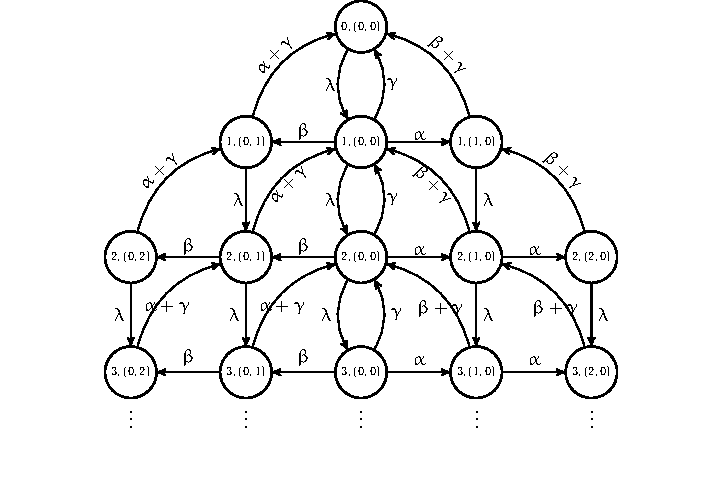
\includegraphics[scale=1,trim= 1.5cm 1cm 1.5cm 0cm]{MatrixAnalytics}
%     \caption{Truncated Markov chain corresponding to the problem in Fig.~\ref{fig:fig_simplex_t_1_mp__high_traff_aprox}}
%     \label{fig:fig_simplex_t_1_truncated_mp_matrix_analytics}
%   \end{center}
% \end{figure}
In order to solve the above system, we assume the steady-state probability vectors to be of the form,
\begin{equation}
  \bm{\pi}_i = \bm{\pi}_1\bm{R}^{i-1}, \quad i \geq 1.
  \label{eq:eq_pi}
\end{equation}
where $\bm{R} \in R^{5 \times 5}$. Combining \eqref{eq:eq_system} and \eqref{eq:eq_pi} we get the following system,
\begin{equation}
  \begin{split}
  & \bm{\pi}_0\bm{F}_0 + \bm{\pi}_1\bm{L}_0 = 0 \\
  & \bm{\pi}_0\bm{H}_0 + \bm{\pi}_1(\bm{F} + \bm{RL}) = 0 \\
  & \bm{\pi}_i(\bm{H} + \bm{RF} + \bm{R}^2\bm{L}) = 0, \quad i \geq 1.
  \end{split}
  \label{eq:eq_system2}
\end{equation}
We notice from \eqref{eq:eq_system2} that a common condition for the system to hold is,
\begin{equation}
  \begin{split}
    & \bm{H}+\bm{RF}+\bm{R}^2\bm{L} = \bm{0} \\
	& \bm{R} = -\left(\bm{R}^2\bm{L}+\bm{H}\right)\bm{F}^{-1}
  \end{split}
  \label{eq:eq_R}
\end{equation}

The inverse of $\bm{F}$ in \eqref{eq:eq_R} exists since $\det(\bm{F}) = -\delta^3(\delta-\alpha)(\delta-\beta)\neq 0$ assuming $\lambda > 0$. Using \eqref{eq:eq_R}, an iterative algorithm to compute $\bm{R}$ is given in \ref{alg:alg_R}. The norm $\left||\bm{R}_\textit{i}-\bm{R}_\textit{i-1}\right||$ corresponds to the absolute value of the largest element of the difference matrix $\bm{R}_\textit{i}-\bm{R}_\textit{i-1}$. Therefore, the algorithm ends when the largest difference between the elements of the last two computed matrices is smaller than the threshold $\epsilon$. The initial matrix $\bm{R}_0$ could take any value, not necessarily \bm{0}. The error threshold $\epsilon$ could be fixed to any arbitrary value, but the lower this value the slower the convergence.
\begin{algorithm}
  \caption{Computing matrix $\bm{R}$}\label{alg:alg_R}
  \begin{algorithmic}[1]
  \Procedure{ComputingR}{}
  \State $\epsilon \gets 10^{-6}$
  \State $\bm{R}_0 \gets \bm{0}$
  \State $\textit{i} \gets 1$
  %\State $\bm{R}_1 \gets \bm{0}$
  \While{\bm{true}}
  \State $\bm{R}_i \gets -\left(\bm{R}_{i-1}^2\bm{L}+\bm{H}\right)\bm{F}^{-1}$
  \If{$\left||\bm{R}_\textit{i}-\bm{R}_\textit{i-1}\right||>\epsilon$}
  \State $\textit{i} \gets \textit{i+1}$
  \Else\ \Return $\bm{R}_i$
  \EndIf
  \EndWhile
  \EndProcedure
  \end{algorithmic}
\end{algorithm}

Computing $\bm{R}$, the vectors $\bm{\pi}_0$ and $\bm{\pi}_1$ are remaining to be found in order to deduce the values of all limiting probabilities. To solve this problem, recall that in \eqref{eq:eq_system2} there are still the first two equations to be used. Writing these two equations in matrix form,
\begin{equation}
  \label{eq:eq_finding_pi0_pi1_1}
  \left[\begin{array}{cc}
  \bm{\pi}_0 & \bm{\pi}_1
  \end{array}\right]\left[\begin{array}{cc}
  \bm{F}_0 & \bm{H}_0\\
  \bm{L}_0 & \bm{RL}+\bm{F}
  \end{array}\right]=\bm{0},
\end{equation}
where $\bm{0}$ is a $1 \times 9$ zeros vector and $\Phi=\left[\begin{array}{cc}
\bm{F}_0 & \bm{H}_0\\
\bm{L}_0 & \bm{RL}+\bm{F}
\end{array}\right]$ is a $9 \times 9$ matrix. In addition, we also have the normalization equation to take into account. Denoting $\bm{1}_0=[1, 1, 1, 1]$, $\bm{1}_1=[1, 1, 1, 1, 1]$ and using \eqref{eq:eq_pi}, we obtain,
\begin{align}
  \label{eq:eq_norm}
  \bm{\pi}_0\bm{1}_0^T + \sum_{i=1}^\infty \bm{\pi}_i\bm{1}_1^T &= 1 \\
  \bm{\pi}_0\bm{1}_0^T + \sum_{i=1}^\infty \bm{\pi}_1\bm{R}^{i-1}\bm{1}_1^T &= 1 \\
  \bm{\pi}_0\bm{1}_0^T + \bm{\pi}_1(\sum_{i=1}^\infty \bm{R}^{i-1})\bm{1}_1^T &= 1 \\
  \bm{\pi}_0\bm{1}_0^T + \bm{\pi}_1(\bm{I}-\bm{R})^{-1}\bm{1}_1^T &= 1 \\
  \left[\begin{array}{cc}
  \bm{\pi}_0 & \bm{\pi}_1
  \end{array}\right]\left[\begin{array}{c}
  \bm{1}_0^T \\
  \left(\bm{I}-\bm{R}\right)^{-1}.\bm{1}_1^T
  \end{array}\right] &= 1,
\end{align}
where $\bm{I}$ is the $5 \times 5$ identity matrix. In order to find $\bm{\pi}_0$ and $\bm{\pi}_1$, we solve the following system 
\begin{align}
\label{eq:eq_system_final}
\left[\begin{array}{cc}
\bm{\pi}_0 & \bm{\pi}_1
\end{array}\right]\Psi &= \left[1, 0, 0, 0, 0, 0, 0, 0, 0\right],
\end{align}
where $\Psi$ is obtained by replacing the first column of $\Phi$ with $[\bm{1}_0, \bm{1}_1(\bm{I}-\bm{R}^T)^{-1}]^T$. Hence, \eqref{eq:eq_system_final} is a linear system of $9$ equations with $9$ unknowns. After solving \eqref{eq:eq_system_final}, we obtain the remaining limiting probabilities vector using \eqref{eq:eq_pi}.
% $\left[\begin{array}{c}
% \bm{1}_0^T\\
% \left(\bm{I}-\bm{R}\right)^{-1}.\bm{1}_1^T
% \end{array}\right]$

\subsubsection{Approximating the average system time $E[T]$}
Once the limiting probabilities computed, we can use these results in order to calculate the average system time $E[\hat{T}_{MA}]$ of the truncated version of the Markov chain in Fig.~\ref{fig:fig_simplex_t_1_mp__high_traff_aprox}. We use Little's theorem which states
\begin{equation}
\label{eq:eq_little_thm}
  E[\hat{T}_{MA}] = \frac{E[\hat{N}_{MA}]}{\lambda},
\end{equation}
where $N_{MA}$ is the total number of jobs in the system. In order to calculate the average number of jobs in the system we first notice that
\begin{equation*}
  \begin{split}
    Pr\{N=0\} &= \pi_{0,(0,0)} \\
	Pr\{N=1\} &= \pi_{1,(0,0)} + \pi_{1,(0,1)} + \pi_{1,(1,0)} = \bm{\pi}_0\bm{1}_0^T-\pi_{0,(0,0)} \\
	Pr\{N=i\} &= \pi_{i,(0,2)} + \pi_{i,(0,1)} + \pi_{i,(0,0)}+ \pi_{i,(1,0)} + \pi_{i,(2,0)} = \bm{\pi}_{i-1}\bm{1}_1^T, \quad i \geq 2.
  \end{split}
\end{equation*}
Therefore, one can compute $E[\hat{N}_{MA}]$ as
\begin{equation}
  \begin{split}
  E[&\hat{N}_{MA}] = \sum_{i=0}^{\infty} i Pr\{N_{MA}=i\} \\
    &= \bm{\pi}_0\bm{1}_0^T-\pi_{0,(0,0)} + \sum_{i=2}^{\infty} i(\bm{\pi}_{i-1}\bm{1}_1^T) \\
    &= \bm{\pi}_0\bm{1}_0^T-\pi_{0,(0,0)} + \sum_{i=2}^{\infty} i(\bm{\pi}_1\bm{R}^{i-2}\bm{1}_1^T) \\
    &= \bm{\pi}_0\bm{1}_0^T-\pi_{0,(0,0)} + \bm{\pi}_1 (\sum_{i=2}^{\infty} i \bm{R}^{i-2})\bm{1}_1^T \\
    &= \bm{\pi}_0\bm{1}_0^T-\pi_{0,(0,0)} + \bm{\pi}_1 (\sum_{i=2}^{\infty} (i-1)\bm{R}^{i-2} + \bm{R}^{i-2})\bm{1}_1^T \\
    &= \bm{\pi}_0\bm{1}_0^T-\pi_{0,(0,0)} + \bm{\pi}_1 (\sum_{j=1}^{\infty} j\bm{R}^{j-1} + \sum_{i=0}^{\infty} \bm{R}^i)\bm{1}_1^T \\
    &= \bm{\pi}_0\bm{1}_0^T-\pi_{0,(0,0)} + \bm{\pi}_1 ((\bm{I}-\bm{R})^{-2} + (\bm{I}-\bm{R})^{-1})\bm{1}_1^T.
  \end{split}
  \label{eq:eq_avgN}
\end{equation}
Using (\ref{eq:eq_little_thm}) and (\ref{eq:eq_avgN}) we deduce the average system time $E[\hat{T}_{MA}]$.

\subsubsection{Results and simulations} Equation \eqref{eq:eq_avgN} shows that we only need $\bm{\pi}_0$, $\bm{\pi}_1$ and $\bm{R}$ in order to compute the average system time. Hence, no need  to calculate infinite number of limiting probabilities. It is worth noting that the calculated average system time $E[\hat{T}_{MA}]$ is an upper bound of the actual average system time $E[T]$ corresponding to the system in Fig.~\ref{fig:fig_simplex_t_1_mp__high_traff_aprox}. Indeed, the truncated Markov chain is equivalent to imposing a blocking on the repair group whenever one of the server leads by 2 jobs. Comparison with the simulation given in Fig.~\ref{fig:fig_simplex_t_1_matrix_analytic_ub} confirms this fact. 
\begin{figure}[h]
  \centering
  \includegraphics[width=0.5\textwidth, keepaspectratio=true]{fig_simplex_t_1_matrix_analytic_ub.png}
  \caption{Split-merge upper bound $E[\hat{T}_{SM}]$, upper bound $E[\hat{T}_{MA}]$ obtained using the matrix analytic approach on the truncated MC in Fig.~\ref{fig:fig_simplex_t_1_truncated_mp_matrix_analytics}, simulation $E[T]$ and the M/G/1 lower-bound $E[\hat{T}_{LB}]$ for the average system time in Simplex($t=1$).}
  \label{fig:fig_simplex_t_1_matrix_analytic_ub}
\end{figure}

% \end{comment}
% ############################################  Simplex(t)  ######################################### %
\section{Simplex queue with multiple repair groups}
\label{sec:sec_simplex_avg_sys_time}
Extending the approach presented in Subsection \ref{subsec:subsec_simplex_t_1} for simplex setup with multiple repair groups, i.e., Simplex($t > 1$) is tedious for $t=2$ and not possible for $t > 2$ since the state space complexity exponentially increases with $t$. First, we will show the extension for $t=2$, and then discuss a general lower-bound for expected system time for any value of $t$.

% ------------------------------------------  Simplex(t=2)  ----------------------------------------- %
\subsubsection{A lower-bound for the expected hot-data download time in Simplex($t=2$)}
\label{subsec:subsec_lb_simplex_t_2}
% TODO: Fill in the blanks
Following the job start definition given in Subsection~\ref{subsec:subsec_simplex_t_1} i.e., define job service start time once all its tasks are in service, for $t=2$ there are three types of job starting setups (1) Complete-start: all tasks of the job starts service simultaneously, (2) Partial-start of the \nth{1} kind (partial-$1$): one task in one of the repair groups finishes service early and the remaining the rest of the tasks of the job start service simultaneously, (2) Partial-start of the \nth{2} kind (partial-$2$): two separate tasks in two repair groups finish service early and the rest of the tasks of the job start service simultaneously. Job service time distributions for each starting setup are as follows; (1) for complete-start, $V_c = min\{Exp(\lambda),\max\{Exp(\mu),Exp(\mu)\},\max\{Exp(\mu),Exp(\mu)\}\}$, (2) for partial-$1$ start, $V_{p_1} = \min\{Exp(\lambda),Exp(\mu),\max\{Exp(\mu),Exp(\mu)\}\}$, (3) for partial-$2$ start, $V_{p_2} = \min\{Exp(\lambda),Exp(\mu),Exp(\mu)\}$. First and second moments of the service time for each starting setup can be calculated easily from the first principles.

Simplex($t=2$) can be modeled as an M/G/1 queue and PK formula can be used to get a lower-bound as the one found for Simplex($t=1$) in \eqref{eq:eq_simplex_t_1_lb}. This requires finding $E[V]$ and second $E[V^2]$ moments for service time of an arbitrary job, similar to \eqref{eq:eq_simplest_simplex_serv_time_moments} one can write the following.
\begin{equation}
  \label{eq:eq_simplex_t_2_moments}
  \begin{split}
    & E[V] = f_J(c)E[V_c] + f_J(p_1)E[V_{p_1}] + f_J(p_2)E[V_{p_2}] \\
    & E[V^2] = f_J(c)E[V_c^2] + f_J(p_1)E[V_{p_1}^2] + f_J(p_2)E[V_{p_2}^2]
  \end{split}
\end{equation}

System state space for general arrival regime is not tractable, thus we try to estimate the limiting probability $f_J(j)$ of a job making start type $j$ by studying the system under high-traffic regime. As in Subsection~\ref{subsec:subsec_simplex_t_1}, imagine a join queue at the tail of the system, in which the tasks that finish service wait for their siblings to finish service. In each repair group, only one server can be ahead with the task completion since a task completion from the slow server will signal the job completion. Suppose the service rate at the systematic server is $\gamma$ and the service rate of each repair server is $\mu$. Since the repair servers are same and there is no need to distinguish the leading server in a repair group, state of the join queue can be defined as $\bm{n}(t) = (n_1(t), n_2(t))$ where $n_i$ denotes the number of tasks that departed from the leading server at repair group $i$ and are waiting in the join queue at time $t$. Under the high-traffic regime, $\bm{n}(t)$ is a Markov process which is shown in Fig.~\ref{fig:fig_simplex_t_2_mp_high_traff}. 
\begin{figure}[htb]
  \centering
  \begin{tikzpicture}
    \node at (0,0)  {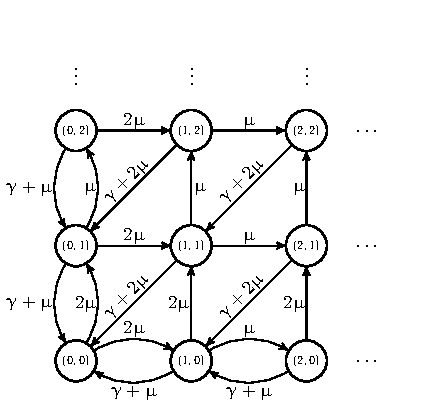
\includegraphics{simplex_t_2_mp} };
  \end{tikzpicture}
  \vspace*{-0.2cm}
  \caption{Markov process for Simplex(t=2) under high-traffic assumption.}
  \label{fig:fig_simplex_t_2_mp_high_traff}
\end{figure}

Using the embedded MC within the Markov process in Fig.~\ref{fig:fig_simplex_t_2_mp_high_traff} will allow us to find estimates $f_{jc}$, $f_{jp_1}$ and $f_{jp_2}$ for respectively $f_J(c)$, $f_J(p_1)$ and $f_J(p_2)$. Following the same arguments discussed for Simplex($t=1$) in finding \eqref{eq:eq_simplest_simplex_est_serv_time_moments}, we can compute the estimates $E[\hat{V}]$ and $E[\hat{V}^2]$ for $E[V]$ and $E[V^2]$ as in \eqref{eq:eq_simplex_t_2_est_serv_time_moments}. These estimates are lower-bounds as can easily be seen given that $E[V_c] > E[V_{p_*}]$, and $f_{jc} < f_J(c)$, $\sum_{i}f_{jp_i} > \sum_{i}f_J(p_i)$ .
\begin{equation}
  \label{eq:eq_simplex_t_2_est_serv_time_moments}
  \begin{split}
    & E[\hat{V}] = f_{jc}E[V_c] + f_{jp_1}E[V_{p_1}] + f_{jp_2}E[V_{p_2}] < E[V] \\
    & E[\hat{V}^2] = f_{jc}E[V_c^2] + f_{jp_1}E[V_{p_1}^2] + f_{jp_2}E[V_{p_2}^2] < E[V^2]
  \end{split}
\end{equation}

Steady-state state probabilities $\pi_{i,j}$ for the embedded MC is equal to $p_{i,j}$ since the total transition rate out of every state is equal to $\nu=\gamma+4\mu$. Under high-traffic assumption, after every job departure at time $\tau$, a new job starts service at $\tau^+$ so the starting setup for the new job is determined by $\bm{n}(\tau)$. Therefore, defining the limiting fraction of state transitions corresponding to job departures as $f_{jd}$, those into a complete-start state as $f_c$, and those into a partial-i-start state as $f_{p_i}$, one can compute $f_{jc}$, $f_{jp_1}$ and $f_{jp_2}$ as below.
\begin{equation}
  \label{eq:eq_simplex_t_2_start_setup_fracs}
  \begin{split}
    & \begin{aligned}
      f_{jd} &= \frac{\gamma}{\nu}\pi_{0,0} + \frac{\gamma+\mu}{\nu}\sum_{i=1}^{\infty}(\pi_{0,i}+\pi_{i,0}) \\
      &+ \frac{\gamma+2\mu}{\nu}(1-\pi_{0,0}-\sum_{i=1}^{\infty}(\pi_{0,i}+\pi_{i,0})),
    \end{aligned} \\
    & f_c = \frac{\gamma}{\nu}\pi_{0,0} + \frac{\gamma+\mu}{\nu}(\pi_{0,1}+\pi_{1,0}) + \frac{\gamma+2\mu}{\nu}\pi_{1,1}, \\
    & f_{p_1} = \frac{\gamma+2\mu}{\nu}\sum_{i=2}^{\infty}(\pi_{i,2}+\pi_{2,i}), \\
    & f_{jc} = \frac{f_c}{f_{jd}}, \quad f_{jp_1} = \frac{f_{p_1}}{f_{jd}}, \quad f_{jp_2} = 1-f_{jc}-f_{jp_1}.
  \end{split}
\end{equation}

% Intuitively, in simplex queue under stability the Markov process is recurrent, which requires the system to regularly visit idle state.
\mehmet{For now dropped on showing a stability criterion for processes for t=1,2. Foster's theorem and Rosenberg's extension of it for multidimensional chains can be applied to find a stability criterion or to formalize the observation below. A very good relevant paper: Stability Conditions for Multidimensional Queueing Systems and Applications to Analysis of Computer Systems}
Markov process in Fig.~\ref{fig:fig_simplex_t_2_mp_high_traff} is hard to analyze. It is irreducible and for recurrence, $p_{i,j}$ of should decrease with $i$ and $j$. One can see this from the simulation or from the following informal argument. Expected drift at $(i,j),~i,j>0$ (i.e., inner states) towards $(i-1,j-1)$ is greater than the drift towards $(i+1,j)$ and $(i,j+1)$. Expected drift at $(i,0),~i>0$ (i.e., states at the horizontal boundary) towards $(i-1,0)$ and $(i,1)$ is greater than the drift towards $(i+1,0)$. Similar observation can be made for the states at the vertical boundary. Therefore, we expect the system to spend more time in the lower-left region of the state-space, which gives us the idea of truncating the process and working with the truncated version. To keep the transition probabilities within the embedded MC same, we define the truncation as follows. Suppose the transition probability matrix of $\bm{n}(t)$ is $\bm{P}$ and the truncated process is $\bm{\tilde{n}}(t)=\{(i,j) | i,j \leq M\}$ where $M$ defines the boundary where the truncation starts. Then the transition probability matrix $\bm{\tilde{P}}$ of $\bm{\tilde{n}}(t)$ is defined as
\begin{equation*}
  \bm{\tilde{P}}_{i,j} =
  \begin{cases}
    0,        				      & j > M, i \leq M, \\
    \sum_{j \geq M} \bm{P}_{i,j}, & j=i \leq M, \\
    \bm{P}_{i,j},  				  & j \leq M, i \leq M.
  \end{cases}
\end{equation*}
One important consequence of truncation is that $\tilde{\pi}_{i,j}$ for the MC embedded within $\bm{\tilde{n}}(t)$ will have higher values for the remaining states i.e., $\tilde{\pi}_{i,j} > \pi_{i,j},~i,j \leq M$. Think of the truncated chain with the two disjoint set of nodes $S_K = \{(i,j)|\min\{i,j\} \leq K\}$ and $S^\prime_K = \bm{\tilde{n}}(t)/S_K$ where $K > 0, i,j \leq M$. Observe that transitions between $S_K$ and $S^\prime_K$ exist only between the nodes that are on boundaries $B_K = \{(i,j)|\min\{i,j\}=K\}$ and $B_{K+1}$. Using Theorem 12.13 in \cite{yates1999probability}, we have by letting $\Sigma_K = \sum_{(i,j) \in B_K} \pi_{i,j}$ and total departure rate from each state $\nu = \gamma+4\mu$,
\begin{equation*}
  \begin{split}
  & (\Sigma_0 - \pi_{0,0}) \frac{2\mu}{\nu} = \Sigma_1 \frac{\gamma+2\mu}{\nu}, \\
  & (\Sigma_i - \pi_{i,i}) \frac{\mu}{\nu} = \Sigma_{i+1} \frac{\gamma+2\mu}{\nu}; ~i > 0, \\
  & \text{Define } \rho = 2 + \frac{\gamma}{\mu}, \\
  & \Sigma_0 \geq \frac{\rho}{2}\Sigma_1 \text{ and } \Sigma_i \geq \rho\Sigma_{i+1}; ~i > 0.
  \end{split}
\end{equation*}
Next think of the truncated chain with the two disjoint set of nodes $S_K = \{(i,j)|i,j \leq M\}$ and $S^\prime_K = \bm{\tilde{n}}(t)/S_K$ where $K > 0, i,j \leq M$. Observe that transitions between $S_K$ and $S^\prime_K$ exist only between the nodes that are on boundaries $C_K = \{(i,j)|\max\{i,j\}=K\}$ and $C_{K+1}$. We have by letting $\sigma_K = \sum_{(i,j) \in C_K} \pi_{i,j}$
\begin{equation*}
  \begin{split}
%   & \sum_{n \in S}\sum_{n^\prime \in S^\prime} \pi_{n}P_{n,n^\prime} = \sum_{n^\prime \in S^\prime}\sum_{n \in S} \pi_{n^\prime}P_{n^\prime,n} \\
%   & \sum_{n \in S} \pi_{n} \sum_{n^\prime \in S^\prime} P_{n,n^\prime} = \sum_{n^\prime \in S^\prime} \pi_{n^\prime} \sum_{n \in S} P_{n^\prime,n} \\
  & (\sigma_0 - \pi_{0,0}) \frac{2\mu}{\nu} \geq \sigma_1 \frac{\gamma+\mu}{\nu}, \\
  & (\sigma_i - \pi_{i,i}) \frac{\mu}{\nu} \geq \sigma_{i+1} \frac{\gamma+\mu}{\nu}, \\
  & \text{Define } \tau = 1 + \frac{\gamma}{\mu}, \\
  & \sigma_0 \geq \frac{\tau}{2}\sigma_1 \text{ and } \sigma_i \geq \tau \sigma_{i+1}; ~i > 0.
  \end{split}
\end{equation*}
Overall for any $M > 0$, $\Sigma_i$ and $\sigma_i$ at least exponentially decrease with $i$. This is suggesting that $\tilde{\pi}_{i,j} - \pi_{i,j}$ due to truncation will be higher for lower $i,j$ because the lower-left region of the chain is weighted exponentially more i.e., lower-left region gets higher share of increase. As can be seen in \eqref{eq:eq_simplex_t_2_start_setup_fracs}, $f_{jc}$ and $f_{jp_1}$ are functions of $\tilde{\pi}_{i,j}$ for states in the lower-left region. Therefore, the truncated chain gives higher values for $f_{jc}$ and $f_{jp_1}$, thus there is no guarantee that the M/G/1 model will be always a lower-bound in this case.

We can solve the truncated chain~\footnote{Solving the truncated chain analytically is tedious but steady-state probabilities can be computed easily with a computer} to compute $f_{jc}$, $f_{jp_1}$, $f_{jp_2}$ and plugging them into \eqref{eq:eq_simplex_t_2_est_serv_time_moments} will give us everything to write the lower-bound $E[\hat{T}_{LB}]$ using the PK formula. Fig.~\ref{fig:fig_simplex_t_2_truncated_high_traff_chain_ub_lb} compares $E[\hat{T}_{LB}]$ attained by setting the truncation index $M=5$ and $M=2$, and simulated $E[T]$. Lower-bound obtained by $M=5$ using the high-traffic regime assumption performs pretty good for Simplex($t=2$). Note that as discussed in the previous paragraph, when $M$ is low, the model becomes an upper bound after threshold in arrival rate is crossed as shown for $M=2$ on the plot. Thus, the model for lower values of $M$ can be used only as an approximation and do not imply a bound.
\begin{figure}[h]
  \centering
  \includegraphics[width=0.5\textwidth, keepaspectratio=true]{fig_simplex_t_2_truncated_high_traff_chain_ub_lb.png}
  \caption{Split-merge upper-bound $E[\hat{T}_{SM}]$, the M/G/1 lower-bound $E[\hat{T}_{LB}]$ attained by setting $M=2$ and $M=5$, and the simulated $E[T]$ for the average system time in Simplex($t=2$).}
  \label{fig:fig_simplex_t_2_truncated_high_traff_chain_ub_lb}
\end{figure}

% -------------------------  A LB with the Conjecture and Renewal Theory for Simplex(t) ------------------------- %
\subsection{A general lower-bound for the expected hot-data download time in simplex queue}
\label{subsec:subsec_simplex_t_lb_conjecture_renewals}
Previously we saw that an M/G/1 model using high-traffic assumption and computing the moments for job service completion time given varying service starting setups performs well for simplex queue with one and two repair groups. Unfortunately, the process for the join queue becomes very tedious quickly as we experienced with the Simplex($t=2$). Generalizing this analysis to systems with higher number of repair groups is simply formidable. In this section, we try to find lower-bounds by using the observations collected from the analysis of simplex queue for $t=1$ and $t=2$. Note that throughout the discussion, we continue using the high-traffic assumption under which queues are never empty.

We start by generalizing some of the terminology used previously. Suppose the service time at each repair server is $Exp(\mu)$ and at systematic server it is $Exp(\gamma)$. Given this setup, we index all possible starting types (instead of calling them complete and partial) starting from $0$ up to $t$ where type-$i$ setup means that at the job starting instant, only one task of the job is in service at $i$ repair groups while in the other $t-i$ repair groups both sibling tasks are in service. Given this definition, complete-start is equivalent to type-$0$ start. First and second moments $E[S_i]$, $E[S_i^2]$ for the job service completion time for type-$i$ starting setup can be calculated as follows:
\begin{equation}
\label{eq:eq_job_starting_setup_moments}
  \begin{split}
    & Pr\{S_i \geq s\} \\
    &= Pr\{S_{\gamma} \geq s\}Pr\{S_{\mu} \geq s\}^i Pr\{\max\{S_{\mu}, S_{\mu}\} \geq s\}^{t-i} \\
    &= e^{-\gamma s}e^{-i\mu s}(1-(1-e^{-\mu s})^2)^{t-i} \\
    &= e^{-(\gamma+t\mu)s}(2-e^{-\mu s})^{t-i} \\
    &= e^{-(\gamma+t\mu)s} \sum\limits_{k=0}^{t-i} {{t-i}\choose{k}} 2^k (-e^{-\mu s})^{t-i-k} \\
    &= \sum\limits_{k=0}^{t-i} {{t-i}\choose{k}} 2^k (-1)^{t-i-k} e^{-(\gamma+\mu(2t-i-k))s} \\
    & E[S_i] = \int_{0}^{\infty} Pr\{S_i \geq s\} ds \\
    &= \sum\limits_{k=0}^{t-i} {{t-i}\choose{k}} 2^k (-1)^{t-i-k} \frac{1}{\gamma+\mu(2t-i-k)} \\
    & E[S_i^2] = \int_{0}^{\infty} 2s Pr\{S_i \geq s\} ds \\
    &= \sum\limits_{k=0}^{t-i} {{t-i}\choose{k}} 2^k (-1)^{t-i-k} \frac{2}{(\gamma+\mu(2t-i-k ))^2}
  \end{split}
\end{equation}

Intuitively, $E[S_i]$ should monotonically decrease with $i$ because type-$i$ start means at $i$ repair groups, one sibling task already finished service that is to call the job done, only one task is left to serve in these leading repair groups which is better than having to wait for both sibling tasks to be serviced. In the following, we establish that $E[S_i]$ monotonically decreases with $i$.
\begin{equation}
  \begin{split}
    & E[S_i - S_{i+1}] = \int_{0}^{\infty} (Pr\{S_i \geq s\} - Pr\{S_{i+1} \geq s\})ds \\
    &= \lim_{\Delta \to 0} \sum\limits_{k=0}^{\infty} (Pr\{S_i \geq k\Delta\} - Pr\{S_{i+1} \geq k\Delta\})\Delta \\
    &= \lim_{\Delta \to 0} \sum\limits_{k=0}^{\infty} e^{-(\gamma+t\mu)k\Delta}((2-e^{-\mu k\Delta})^{t-i} - (2-e^{-\mu k\Delta})^{t-i-1})\Delta \\
    &> 0
  \end{split}
\end{equation}
where $(2-e^{-\mu k\Delta})^{t-i} - (2-e^{-\mu k\Delta})^{t-i-1} > 0$ since $2-e^{-\mu k\Delta} > 1$. Same thing can be carried out to see that $E[S_i^2]$ monotonically decrease with $i$. \mehmet{Here we may show and discuss that $E[S_i]$ and $E[S_i^2]$ follow the "diminishing return" which can be used to argue that adding more multiple repair groups yield diminishing returns in terms of reducing the data access time.}

We previously observed for $t=1,2$ that the fraction of the jobs that make type-$i$ start decrease with $i$. This can be explained with the following informal argument. For type-$i$ start, at the job starting time instant, system should have $i$ repair groups with a \emph{leading} server that already finished servicing the assigned task of the job -- we call such groups as "leading groups", and have the other $t-i$ non-leading groups in which both servers can start serving the sibling tasks of the job. For a repair group, it is less likely to be leading because every job termination helps the slow servers to catch up with the leading server. Remember that completion of a job allows the slow servers that are still working on the assigned tasks of the completed job to cancel the task and proceed with the next task waiting in the queue. In simplex queue, job termination can be signaled by the systematic server or by any repair group, while a leading server alone should serve faster and compete with every other server to keep leading. Overall, it is intuitively expected to have more jobs making type-$i$ start for lower values of $i$.

Next, we try to state what is informally argued in the previous paragraph in a slightly more formal way. Define $L_k(t)$ as the number of tasks that the leading server at repair group $k$ is leading by at time $t$. Suppose $j$th job makes a type-$i$ start at time $\tau$, namely $J_j = i$. We have the following inequality $Pr\{J_{j+1} > i|J_j=i, A\} > Pr\{J_{j+1} > i|J_j=i\}$ where $A$ denotes the event that $L_k(\tau) > 1$ for every leading repair group $k$. Event $A$ guarantees $J_{j+1} \geq i$ i.e., $Pr\{J_{j+1} \geq i|J_j=i, A\}=1$, since even in case none of the leading servers advances before $j$th job gets completed, next job will make at least type-$i$ start. We will try to compute $Pr\{J_{j+1} > i|J_j=i, A\} = 1 - Pr\{J_{j+1}=i|J_j=i, A\}$. Suppose $j$th job gets completed at time $\tau^\prime$ and without loss of generality repair group $k$ is leading if $k \leq i$ and non-leading otherwise. Events $\{J_{j+1}=i|J_j=i, A\}$ and $B_i = \{L_k(\zeta) < 2; \zeta \in [\tau, \tau^\prime], i < k \leq t\}$ for $0 < i < t-1$ are equivalent since for $(j+1)$th job to make type-$(i+1)$ start, in at least one of the non-leading repair groups a server should advance by at least $2$ tasks before $j$th job gets completed. Event $B_i$ can also be expressed as $\bigcup\limits_{l=0}^{t-i} C_l$ where $C_l = \{L_{k_j}(\tau)=1; 1 \leq j \leq l, i < k_j \leq t\}$. Event $C_l$ describes that $l$ non-leading repair groups start leading by $1$ before $j$th job terminates. Given that there exists $i$ leading groups, denote the probability of an event that a new repair group starts to lead by $1$ as $p_i^{+1}$ and of the event that $j$th job terminates as $p_i^T$, so we can write $Pr\{C_l\} = p_{i+l}^T\prod\limits_{k=i}^{i+l-1}p_k^{+1}$. Since events $C_l$ for $0 \leq l \leq t-i$ are disjoint, $Pr\{B_i\} = \sum\limits_{l=0}^{t-i} Pr\{C_l\}$ from which we can get the recurrence relation $Pr\{B_i\} = p_i^T + p_i^{+1}Pr\{B_{i+1}\}$. Since service times at the servers are assumed Exponential, probabilities are easy to find as $p_i^T = (\gamma+i\mu)/(\gamma+2t\mu)$ and $p_i^{+1} = (2(t-i)\mu)/(\gamma+2t\mu)$ where $\gamma$ and $\mu$ are respectively service rates of the systematic server and any server in repair groups.

Consider the homogeneous case where $\gamma=\mu$, which gives $p_i^T = (i+1)/(2t+1)$ and $p_i^{+1} = 2(t-i)/(2t+1)$. We find
\begin{equation}
  \begin{split}
    Pr\{B_{t-1}\} &= p_{t-1}^T + p_{t-1}^{+1}p_t^T \\
    &= \frac{t}{2t+1} + \frac{2}{2t+1}\frac{t+1}{2t+1} \\
    &= 1 - \frac{t}{2t+1} + \frac{1}{(2t+1)^2} > \frac{1}{2}
  \end{split}
\end{equation}
Then suppose $Pr\{B_{k+1}\} > 0.5$
\begin{equation}
  \begin{split}
    Pr\{B_k\} &= \frac{k+1}{2t+1} + \frac{2(t-i)}{2t+1}Pr\{B_{k+1}\} \\
    &> \frac{k+1}{2t+1} + \frac{t-k}{2t+1} \\
    &= \frac{t+1}{2t+1} = \frac{1}{2} + \frac{0.5}{2t+1} > \frac{1}{2}
  \end{split}
\end{equation}
Knowing $Pr\{B_{t-1}\} > 0.5$ together with $Pr\{B_k\} > 0.5$ given that $Pr\{B_{k+1}\} > 0.5$ gives us $Pr\{B_i\} > 0.5$ for each $i$. Remember $Pr\{J_{j+1}=i|J_j=i, A\} = Pr\{B_i\}$, so we find $Pr\{J_{j+1} > i|J_j=i\} < Pr\{J_{j+1} > i|J_j=i, A\} = 1 - Pr\{B_i\} < 0.5$. This tells us that for any job and any type-$i$ starting state, next job is more likely to make type-$(\leq i)$ start. 

This suggests that given the fraction of jobs which make type-$i$ start denoted as $f_i$, we have $f_i > f_{i+1}$. \mehmet{Not really, implemented a simple case where the result above does not imply this; trials fail to hold this inequality for high values of $i$. For now we will keep it as a conjecture.}
% This can be seen more clearly as follows. Think of the system state as the starting setup type of the job that is currently in-service, so state space is $\{0, \ldots, t\}$ where the state transition corresponds to departure of the job in-service and immediate start of the next job's service. 

M/G/1 model for the Simplex system with $t$ repair groups allows us to use PK formula to find the expected system time such that $E[T] = E[V] + \lambda E[V^2]/[2(1 - \lambda E[V])]$. Moments for the job service time are $E[V] = \sum_{i=0}^t f_i E[S_i]$ and $E[V^2] = \sum_{i=0}^t f_i E[S_i^2]$. Finding the actual values for $f_i$ is a hard problem as we observed even for Simplex($t \leq 2$). In the following, we find some bounds on $E[T]$ using some estimates of $f_i$.

Previously we found that $E[S_i]$, $E[S_i^2]$ and $f_i$ monotonically decrease with $i$. We can write the relation $f_i > f_{i+1}$ as $f_{i+1} = \rho_i f_i$ where $\rho_i < 1$ for $0 \leq i \leq t$. Finding exact values of $f_i$ turns into finding the values for $\rho_i$ then using the normalization requirement $\sum_{i=0}^t f_i = 1$ as follows:
\begin{equation}
  \label{eq:eq_job_start_fraction_exact_expressions}
  \begin{split}
    & \sum_{i=0}^t f_i = \sum_{i=0}^t f_0 \prod_{j=0}^{i-1} \rho_j = 1 \text{ gives}, \\
    & f_0 = \frac{1}{\sum_{i=0}^t \prod_{j=0}^{i-1} \rho_j} \text{ and } f_i = f_0 \prod_{j=0}^{i-1} \rho_j.
  \end{split}
\end{equation}
Estimating each $\rho_i$ with an upper bound $\hat{\rho}_i \geq \rho_i$ and solving for $\hat{f}_i$'s guarantee that $\hat{f}_0 \leq f_0$ as can be seen from equation \eqref{eq:eq_job_start_fraction_exact_expressions} above. Since $\hat{f}_i$ must add up to $1$, difference $f_0 - \hat{f}_0$ will be distributed among $\hat{f}_i$'s for $1 \leq i \leq t$. This will have the effect of putting more weight on higher values of $i$, which means $\hat{f}_i \leq f_i$ for $i \leq \tau$ and $\hat{f}_i > f_i$ for $i > \tau$ where $\tau$ denotes a non-negative integer valued threshold. Using the estimates $\hat{f}_i$ in finding an estimate for $E[V]$ yields $E[\hat{V}(\bm{\hat{\rho}})] = \sum_{i=0}^t \hat{f}_i E[S_i] < E[V]$ where $\bm{\hat{\rho}}$ denotes the vector of estimates $\rho_i$'s because $E[S_i]$'s for lower $i$ are weighted less in this sum and we know $E[S_i]$'s monotonically decrease with $i$. Same can be said about the estimate $E[\hat{V^2}(\bm{\hat{\rho}})] = \sum_{i=0}^t \hat{f}_i E[S_i^2] < E[V^2]$.

We can easily observe that the tighter the bound $\hat{\rho}_i$ is on $\rho_i$, the better estimates $E[\hat{V}]$ and $E[\hat{V^2}]$ are. The naive way to estimate is simply setting all $\hat{\rho}_i$'s to 1, which is the maximum value they can attain. Then $\hat{f}_i$'s follow a uniform distribution and becomes equal to $1/(t+1)$. Using these values estimates can be computed as $E[\hat{V}(\bm{1})] = \sum_{i=0}^t E[S_i]/(t+1)$ and $E[\hat{V^2}(\bm{1})] = \sum_{i=0}^t E[S_i^2]/(t+1)$ where $\bm{1}$ denotes all-ones vector, which then can be substituted as $E[V]$ and $E[V^2]$ in the PK formula to yield the lower-bound $E[\hat{T}(\bm{1})]$ for $E[T]$. In Fig.~\ref{fig:fig_simplex_t_renewal_lb_compar_w_sim}, comparison between $E[\hat{T}(\bm{1})]$ and the simulated $E[T]$ is shown.

In the following, we try to improve the estimates $\hat{\rho}_i$. Denote $\rho_{max} = \max\{\rho_0, \rho_1, \ldots, \rho_t\}$ and observe $\hat{\rho}_i \leq \rho_{max}$. We try to find a good upper bound on $\rho_{max}$ and use it as $\hat{\rho}_i$ to get a better lower-bound than $E[\hat{T}(\bm{1})]$ for $E[T]$.

Denote the expected inter-arrival interval time for job arrivals as $E[X] = 1/\lambda$ and the expected job service time as $E[V]$. Under stability, sub-sequence of the job arrivals that see an empty system in Simplex($t$) forms a renewal process (Theorem 5.5.8 in \cite{gallager2013stochastic}). Since Simplex($t$) is an M/G/1 queue, (Theorem 5.5.10 in \cite{gallager2013stochastic}) we can find the expected number of job arrivals $E[J]$ between successive renewal epochs (initiation of busy periods) can be computed as $E[J] = E[X]/(E[X]-E[V])$. Jobs that see an empty system definitely make type-$t$ start while within a busy period any type of start is probable. This observation reveals that $1/E[J]$ is a lower bound for $f_0$. Computing the value of $E[J]$ requires knowing $E[V]$, which we have been trying to estimate because it is hard to find. Therefore, we can use the inequality $f_0 > 1/E[J] > 1/E[J]_{ub}$ where $E[J]_{ub} > E[J]$. We can find an upper bound on $E[J]$ by finding and substituting a lower bound $E[V]_{lb}$ for $E[V]$ as $E[J]_{ub} = E[X]/(E[X]-E[V]_{lb})$. For instance, we can use $E[\hat{V}(\bm{1})]$ that we've found previously as $E[V]_{lb}$ and compute the lower bound $f_0^{lb} = (E[X]-E[V]_{lb})/E[X] < f_0$. 

Firstly, we calculated $\hat{f}_0 = 1/(1+t)$ by setting each $\hat{\rho}_i$ to $1$, for the system in which $\hat{f}_0$ becomes exact (i.e., $f_0 = \hat{f}_0$), the lower bound obtained from renewal theory $(E[X]-E[V])/E[X]$ holds as well under stability. For this system, $E[\hat{V}(\bm{1})]$ becomes the exact $E[V]$ which gives $\hat{f}_0 = 1/(1+t) > (E[X]-E[\hat{V}(\bm{1})])/E[X]$. Secondly, setting each $\hat{\rho}_i$ to $\rho_{max}$ and using the normalization requirement $\sum_{i=0}^t \hat{f}_i = 1$, we find $\hat{f}_i = \rho_{max}^i \hat{f}_0$ where $\hat{f}_0 = (1-\rho_{max})/(1-\rho_{max}^{t+1})$. One can see that $(1-\rho_{max})/(1-\rho_{max}^{t+1}) \geq 1/(1+t)$ for $0 < \rho_{max} < 1$ so we obtain $(1-\rho_{max})/(1-\rho_{max}^{t+1}) > 1/(1+t) > (E[X]-E[\hat{V}(\bm{1})])/E[X]$. Here we obtained a relation between $\rho_{max}$ for which we strive to find a good upper bound, with $\hat{V}(\bm{1})$ that we found as the naive lower-bound for $E[V]$. Next we use this inequality to get an upper bound on $\rho_{max}$ as follows. Unfortunately, solving for $\rho_{max}$ does not give a closed form solution, so to get one we take the limit as $\lim_{t \to \infty} (1-\rho_{max})/(1-\rho_{max}^{t+1}) = 1-\rho_{max} > (E[X]-E[\hat{V}(\bm{1})])/E[X]$, which gives $\rho_{max} < E[\hat{V}(\bm{1})]/E[X]$. However, taking the limit may make this upper-bound on $\rho_{max}$ not accurate for small values of $t$. This inaccuracy may lead the lower-bound we are trying to find for $E[T]$ to be not a lower-bound but only an approximation. As we will see in the following from the simulations, the expression we found as the upper bound for $\rho_{max}$ by taking the limit as $t \to \infty$ yields a lower-bound even for $t=2$, which is the minimum value that $t$ can attain for simplex queues with multiple repair groups.

Now we have $\hat{\rho}_i < \rho_{max} < E[\hat{V}(\bm{1})]/E[X]$ for $0 \leq i \leq t$. Setting each $\hat{\rho}_i$ to the upper bound $E[\hat{V}(\bm{1})]/E[X]$ which is tighter than $1$ is expected to yield a better lower-bound $E[\hat{T}(\bm{\rho_{max}})]$, where $\bm{\rho_{max}} = \rho_{max}\bm{1}$, than $E[\hat{T}(\bm{1})]$ for $E[T]$. Solving for $\hat{f}_i$, computing the estimates $E[\hat{V}(\bm{\rho_{max}})]$, $E[\hat{V}^2(\bm{\rho_{max}})]$ and finally plugging in the PK formula yields $E[\hat{T}(\bm{\rho_{max}})]$. The expected relation $E[\hat{T}(\bm{1})] < E[\hat{T}(\bm{\rho_{max}})] < E[\hat{T}_{LB}]$ can be seen in Fig.~\ref{fig:fig_simplex_t_renewal_lb_compar_w_sim}. An interesting observation from these plots is that the relative gain achieved by $E[\hat{T}(\bm{\rho_{max}})]$ over $E[\hat{T}(\bm{1})]$ improves as the number of repair groups $t$ increases.

\mehmet{Approximation using the renewal theory}
Next, using the same ideas introduced above we obtain an approximation for $E[T]$. Setting $\hat{f}_i = \hat{\rho}_0\hat{f}_0$ for $0 < \hat{\rho}_0 < 1$, then using normalization requirement $\sum_{i=0}^t \hat{f}_i = 1$ one can find $\hat{f}_0 = 1/(1+t\hat{\rho}_0)$. Using the inequality $1/(1+t\hat{\rho}_0) > 1/(1+t) > (E[X]-E[\hat{V}(\bm{1})])/E[X]$, we get an upper bound on $\hat{\rho}_0$ as $\hat{\rho}_0 \leq (E[X] - E[Y])/E[Y]$ where $E[Y] = E[X]-E[\hat{V}(\bm{1})]$. Following the same idea used previously to find $E[\hat{T}(\bm{\rho_{max}})]$, one can substitute this upper bound as $\hat{\rho}_0$ to compute the values of $\hat{f}_i$'s, which then can be used to find estimates for $E[V]$ and $E[V^2]$, and these estimates can be plugged in the PK formula as previously done above. The resulting lower bound will be better than $E[\hat{T}(\bm{1})]$ and worse than $E[\hat{T}(\bm{\rho_{max}})]$.

Fixing $\hat{\rho}_0 = (E[X] - E[Y])/E[Y]$, and setting $\hat{f}_1 = \hat{\rho}_0\hat{f}_0$, $\hat{f}_i = \hat{\rho}_1\hat{\rho}_0\hat{f}_0$ for $1 \leq i \leq t$, one can then find an upper bound for $\hat{\rho}_1$ executing the same steps given above while finding the upper bound for $\hat{\rho}_0$. Normalization requirement gives $\hat{f}_0 = 1/(1+\hat{\rho}_0(1+\hat{\rho}_1(t-1)))$ and it is easy to see $\hat{f}_0 > 1/(1+t) > E[Y]/E[X]$ which yields $\hat{\rho}_1 \leq (E[X]-E[Y](1-\hat{\rho}_0))/(\hat{\rho}_0 E[Y](t-1))$. The same process can be repeated by fixing $\hat{\rho}_0 = (E[X] - E[Y])/E[Y]$ and $\hat{\rho}_1 = (E[X]-E[Y](1-\hat{\rho}_0))/(\hat{\rho}_0 E[Y](t-1))$ to find an upper bound on $\hat{\rho}_2$. To generalize this, fixing $\hat{\rho}_0$, ..., $\hat{\rho}_{i-1}$ to their respective upper bounds, an upper bound for $\hat{\rho}_i$ can be found as follows:
\begin{equation*}
  \hat{\rho}_i \leq \frac{E[X]-E[Y](1+\sum_{k=0}^{i-1} \prod_{l=0}^{k} \hat{\rho}_l)}{E[Y](t-i)\prod_{k=0}^{i-1} \hat{\rho}_k}
\end{equation*}
Finally, setting each $\hat{\rho}_i$ to their respective upper bounds lets us to compute the values of $\hat{f}_i$'s using which estimates for $E[V]$ and $E[V^2]$ can be computed and finally using PK formula approximation $E[\hat{T}(\bm{\rho})]$ for $E[T]$ can be obtained. Note that, this incremental computation of $\hat{\rho}_i$ aims at finding as tight bounds on $\rho_i$ as possible but this process does not guarantee that $E[\hat{T}(\bm{\rho})]$ is a lower-bound but only serves as an approximation. We observe in Fig.~\ref{fig:fig_simplex_t_renewal_lb_compar_w_sim} that $E[\hat{T}(\bm{\rho})]$ is almost equal to $E[T]$ for $t=2$ and for higher values of $t$ it serves as an upper-bound better than $E[\hat{T}_{SM}]$ that is obtained from split-merge approximation. Simulation comparison for Simplex($t=1$) shows that the lower bounds $E[\hat{T}(\bm{1})]$, $E[\hat{T}(\bm{\rho_{max}})]$ and the approximation $E[\hat{T}(\bm{\rho})]$ we found for system with multiple repair groups approximates the average system time for the system with single repair group almost exactly.
\begin{figure*}[h]
  \centering
  \begin{subfigure}[h]{.45\textwidth}
    \centering
    \includegraphics[width=1\textwidth, keepaspectratio=true]{fig_simplex__1_renewal_lb.png}
%     \caption{}
  \end{subfigure}
  \begin{subfigure}[h]{.45\textwidth}
    \centering
    \includegraphics[width=1\textwidth, keepaspectratio=true]{fig_simplex__2_renewal_lb.png}
%     \caption{}
  \end{subfigure}
  \begin{subfigure}[h]{.45\textwidth}
    \centering
    \includegraphics[width=1\textwidth, keepaspectratio=true]{fig_simplex__3_renewal_lb.png}
%     \caption{}
  \end{subfigure}
  \begin{subfigure}[h]{.45\textwidth}
    \centering
    \includegraphics[width=1\textwidth, keepaspectratio=true]{fig_simplex__4_renewal_lb.png}
%     \caption{}
  \end{subfigure}
%   \begin{subfigure}[h]{.45\textwidth}
%     \centering
%     \includegraphics[width=1\textwidth, keepaspectratio=true]{fig_simplex__5_renewal_lb.png}
% %     \caption{}
%   \end{subfigure}
  \caption{Comparison of the upper-bound $E[\hat{T}_{SM}]$ obtained with split-merge assumption, the approximation $E[\hat{T}(\bm{\rho})]$, the lower-bounds $E[\hat{T}(\bm{1})]$, $E[\hat{T}(\bm{\rho_{max}})]$, $E[\hat{T}_{fast-serial}]$ (discussed in the next Subsection) and the simulated system time $E[T]$ for simplex queue where $t$ is the number of repair groups.}
  \label{fig:fig_simplex_t_renewal_lb_compar_w_sim}
\end{figure*}

% -------------------------  A LB similar to Varki-Gauri LB for FJ and MDS, for Simplex(t) ------------------------- %
\subsection{Another general lower-bound for the expected hot-data download time in simplex queue}
\label{subsec:subsec_simplex_t_lb_varki_gauri}
\mehmet{Interesting note: Varki in "Response Time Analysis of Parallel Computer and Storage Systems" defines job waiting, service start times very similar to our type-$i$ starts. Don't forget to include it while explaining our type-$i$ starts.}
In this part, we will present another lower-bound for the expected system time $E[T]$ of Simplex($t$). Main idea is to express the simplex system consisting of multiple sub-systems working in parallel in terms of sub-systems cascaded in serial. Similar type of argument is used in \cite{varki2001response} to find bounds and approximations of the system time in $(n,n)$ fork-join queues. Then the idea is generalized and used to find a lower-bound in \cite{joshi2012coding} for $(n,k)$ fork-join queues. \mehmet{Assuming $(n,n)$ and $(n,k)$ systems are previously explained.} In the following, we will extend the idea introduced in these papers for Simplex($t$) to derive a similar lower-bound as in \cite{joshi2012coding}.

% State-space for the parallel model
The state space for Simplex($t$) can be expressed by states represented as tuples $\bm{n} = (n_0, \bm{n}_1, \ldots, \bm{n}_t)$ where $n_0$ is the number of tasks in systematic server and each tuple $\bm{n}_i = (n_i^{(1)}, n_i^{(2)})$ for $1 \leq i \leq t$ denotes the number of tasks at the sibling servers in the repair group $i$. Since all the repair servers are identical, state can be redefined as $\bm{n} = (n_0, (l_1, n_1), \ldots, (l_t, n_t))$ where $l_i$ is the number of tasks the fast server is leading by and $n_i$ is the number of tasks in the slow server in repair group $i$. Also using the fact that all the repair servers are identical, tuples for the repair groups are ordered with respect to $l_i$ such that $l_1 \geq l_2 \geq \ldots \geq l_t$.

% Explaining the serial model
The time that a job spends in the system can be thought as factored into \emph{phases}. Every arriving job is split into $1+2t$ tasks in which $t$ pairs of tasks are siblings sent to the same repair group. Until the job service is completed, job may have some tasks from some repair groups finishing service earlier. For instance, in Simplex($t=3$), at most $3$ tasks of the job may depart earlier before the job finishes. We call a job being in phase-$i$ if $i$ tasks of the job already departed where phase-$0$ for a job means that all the tasks of the job are in system, waiting or in service. Overall, every job may go through possibly $t+1$ phases, namely phase-$0$, phase-$1$, ..., phase-$t$, where jobs can move from one phase to only the next phase in order and at each phase jobs may finish service and depart before moving to the next phase. For instance, in Simplex($t=3$), a job in phase-$0$ may depart before moving to phase-$1$ if the task at the systematic server finishes service earlier, or similarly a job in phase-$1$ may depart before moving to phase-$2$ if the task at the systematic server or the remaining task at the leading repair group finishes service earlier.

% Equivalence of the serial and parallel models
The system can be thought as one with $i+1$ queues cascaded in serial where jobs in phase-$i$ are present in queue-$i$. We call this view of the system as the \emph{serial model} while we refer to the structural view of the simplex queue as the \emph{parallel model}. Jobs arrive to queue-$0$ and may possibly travel along the line of the following queues and the job is said to be in phase-$i$ while it is waiting or in service in queue-$i$ as illustrated in Fig.~\ref{fig:fig_simplex_t_serial_model}. Let $N_i$ represent the number of jobs in queue-$i$ which by construction represents the number of jobs in phase-$i$. Then the state space of the serial model consists of tuples $(N_0, \ldots, N_t)$. Service time distribution $S_i$ at the server in queue-$i$ and after departing queue-$i$ the probability that the job leaves the system ($P_{i \rightarrow exit}$) or moves to queue-$i+1$ ($P_{i \rightarrow i+1}$) depends on $N_{i+1}, \ldots N_t$. For instance for Simplex($t=2$), if $N_0 > 0$, $N_1 = N_2 = 0$ at the systematic server $S_i ~ Exp(\gamma+4\mu)$, $P_{i \rightarrow exit} = \gamma/(\gamma+4\mu)$, $P_{i \rightarrow i+1} = 4\mu/(\gamma+4\mu)$ while if $N_0 > 0$, $N_1 = N_2 = 1$ $S_i ~ Exp(\gamma+\mu)$, $P_{i \rightarrow exit} = \gamma/(\gamma+\mu)$, $P_{i \rightarrow i+1} = \mu/(\gamma+\mu)$. In general, $S_i ~ Exp(\mu_i)$ with $\mu_i$ varying between $\gamma+\mu$ and $\gamma + i\mu + 2(t-i)\mu$ by increments of $\mu$.
% As in \cite{varki2001response}, we use ";" as the separator here between state elements while "," is used for the state of the parallel model.
\begin{figure*}[h]
  \centering
  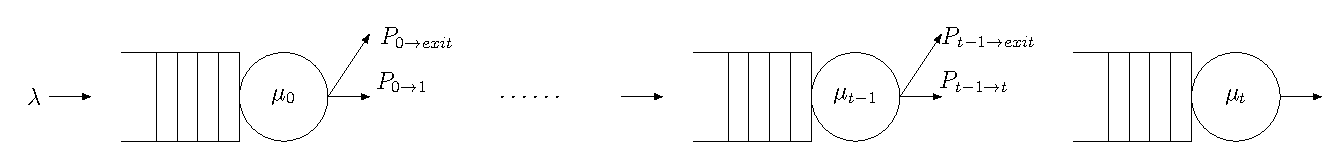
\includegraphics[scale=0.75]{fig_simplex_t_serial_model}
  \caption{Representation of the serial model for Simplex($t$).}
  \label{fig:fig_simplex_t_serial_model}
\end{figure*}

Next with a rather "graphical" argument (i.e., imagining the Markov chain for the parallel and serial models), we argue that the parallel model and the serial model we constructed above are equivalent. By construction, parameters $n_i$ and $l_i$ composing the state space of the parallel model can be expressed in terms of the parameter $N_i$ composing the state space of the serial model as follows, $n_i = \sum_{k=i}^{t} N_k$, $l_i = \sum_{k=0}^{i-1} N_k$. Note that, $n_0$ is equal to the total number of jobs in the system as $n_i + l_i$ is for each $i$. Following the same argument given in \cite{varki2001response}, there is a one-to-one correspondence between the states of the parallel and serial models. In addition, system dynamics for both models are the same meaning that thinking of the Markov chain for both state space, each transition arc between a pair of states in parallel model is present with the same transition probability for the serial model. Thus these two models are equivalent.

Equivalent serial model for the simplex system does not help much with finding an exact expression for the average system time $E[T]$ but gives a way to find a lower bound. Consider a phase-$i$ job in the system being served at the server in queue-$i$ according to the serial model. What this implies in the parallel model is that among the remaining $1+2t-i$ tasks of the job, at least one of them must be in service or at best all of the tasks can be in service. Thus the service rate $\mu_i$ at the server in queue-$i$ is at most $\gamma + (2t-i)\mu$. Setting all the $\mu_i$'s to their highest possible value results in a system that is faster at serving jobs. Fixing each $\mu_i$, each queue becomes an M/M/1 using Burke's Theorem so an expression for the average system time $E[\hat{T}_{fast-serial}]$ can be easily found, which then can be used as a lower-bound for $E[T]$. Rate of arrivals $\lambda_i$ to queue-$i$ is $\lambda\prod_{k=0}^{i-1}P_{k \rightarrow k+1}$, $P_{i \rightarrow exit} = (\gamma+i\mu)/(\gamma+(2t-i)\mu)$, $P_{i \rightarrow i+1} = 1 - P_{i \rightarrow exit}$ and time that a job spends in queue-$i$ is $1/(\mu_i-\lambda_i)$. Then $E[\hat{T}_{fast-serial}]$ can be found as the following:
\begin{equation}
  \begin{split}
    & E[\hat{T}_{fast-serial}] = \frac{1}{\mu_0-\lambda} + \sum_{i=1}^{t} \frac{P_{i-1 \rightarrow i}}{\mu_i-\lambda_i} \\
    & \begin{split}
      =& \frac{1}{\gamma+2t\mu-\lambda} + \\
      & \sum_{i=1}^{t} (\frac{2(t-i)\mu}{\gamma + (2t-i)\mu}) \frac{1}{\gamma + (2t-i)\mu - \lambda\prod_{k=0}^{i-1} \frac{2(t-k)\mu}{\gamma + (2t-k)\mu}} \\
      &< E[T].
    \end{split}
  \end{split}
\end{equation}
Comparison in Fig.~\ref{fig:fig_simplex_t_renewal_lb_compar_w_sim} shows that $E[\hat{T}_{fast-serial}]$ is a much looser lower bound than $E[\hat{T}(\bm{1})]$ and $E[\hat{T}(\bm{\rho_{max}})]$ especially for higher job arrival rate.

% ############################################  Split-to-one Simplex(t)  ######################################### %
\section{Simplex queue with split-to-one access}
\label{sec:sec_simplex_split_to_one}
Load balancing is the act of managing the resources effectively to supply the demanded service requirements. It is desired for systems which are expected to work under high load. High load that the system experiences can either be \emph{symmetric} throughout the operation lifetime or \emph{asymmetric} in that system may go through phases of high and low loads. For asymmetric load scenario, system may benefit from a dynamic resource provisioning scheme, the simplest of which could have two operational states; one gets activated for low-load while the other is active for the high-load phases. For a distributed storage system, data access schemes are either imposed or limited by the way the data is distributed and encoded over the nodes for reliability. Data access schemes optimized for low-load and high-load may require the data to be encoded every time system switches from one scheme to another. This introduces additional operational complexity, which makes the system more prone to operational errors and couples the problems of addressing reliability and fast content access, which is against the "separation of concerns" principle for system design.

LRC's and especially simplex setup discussed in this paper provides the necessary flexibility in the data encoding layer so that the system can seamlessly implement and switch between different data access strategies. Batch codes have been presented for load balancing purposes \cite{ishai2004batch} and their connections to LRC's is studied \cite{skachek2016batch}. Simplex codes are linear batch codes. Therefore, over the data encoded with the simplex code, load balancing strategy can also be implemented besides fast data access time with redundant requests. In Simplex($t$), the simplest strategy for load balancing, namely split-to-one, is to forward the incoming download requests either to the systematic server or one of the repair groups. Simplex setup allows previously analyzed split-to-all and the newly introduced split-to-one access strategies to be used interchangeably. For example, suppose that the traffic for content in the simplex setup follows an asymmetric load pattern. For the lower-arrival rate regime, split-to-all strategy yields smaller average data access time however with split-to-one strategy system operates under stability over greater range of arrival rate. This may allow system to switch from split-to-all to split-to-one strategy seamlessly when the arrival rate increases beyond the critical point so the system can continue provide service under stability. Comparison between the average system time in Simplex($t=1$) using split-to-all and uniformly split-to-one access strategies is shown in Fig.~\ref{fig:fig_simplex_t_1_split_to_all_vs_split_to_one}. Until arrival rate reaches $~1.5$, split-to-all strategy yields smaller average system. However over the range to right of the critical point for stability with split-to-all, system using split-to-one strategy continues to operate under stability until reaching its own critical point.
\begin{figure}[h]
  \centering
  \includegraphics[width=0.5\textwidth, keepaspectratio=true]{fig_simplex_t_1_split_to_all_vs_split_to_one.png}
  \caption{Comparison of the simulated average system time $E[T]$ for Simplex($t=1$) using split-to-all and split-to-one strategies.}
  \label{fig:fig_simplex_t_1_split_to_all_vs_split_to_one}
\end{figure}

A closed form expression for the average system time $E[T]$ for Simplex($t$) under split-to-one is easier to find for that of split-to-all. Every arriving job is independently sent either to systematic node (repair group-$0$) with probability $p_0$ or repair group-$i$ with probability $p_i$ for $1 \leq i \leq t$. Therefore, given the job arrival process is Poisson($\lambda$), the arrivals to repair group-$i$ follow Poisson($\lambda*p_i$). Then the systematic server is M/M/1 queue with service rate $\gamma$ for which the average system time is $1/(\gamma-\lambda_0)$. Each repair group is a fork-join system of two servers (i.e., FJ-2) with the same service rate $\mu$ for which the average system time using the result in \cite{nelson1988approximate} is $(12-\lambda_i/\mu)/(8(\mu-\lambda_i))$. Putting these together, $E[T]$ is found as
\begin{equation}
  E[T] = \frac{p_0}{\gamma-p_0\lambda} + \sum_{i=1}^{t} p_i\frac{12\mu-p_i\lambda}{8\mu(\mu-p_i\lambda)}
\end{equation}

% #########################################  Appendix  ######################################## %
\section{Appendix}
\subsection{Service rate allocation between systematic and repair servers}
\label{subsec:subsec_deriv_E_T_less_than_zero}
Algebra to show $\frac{\partial E[\hat{T}_{LB}]}{\partial \rho} < 0$ that is discussed in Subsection \ref{subsec:subsec_simplex_t_1_res_alloc} is given here. Define $C = \gamma+2\mu$ and $\rho = \gamma/\mu$, then the followings can be calculated
\begin{equation*}
  \begin{split}
  & f_{jc}=\frac{1}{1+\frac{2}{\rho(\rho+2)}}, \quad\quad \frac{\partial f_{jc}}{\partial \rho} = \frac{4(\rho+1)}{(\rho^2+2\rho+2)^2}, \\
  & E[V_p]=\frac{\rho+2}{C(\rho+1)}, \quad\quad E[V_p^2]=\frac{2}{C^2}(\frac{\rho+2}{\rho+1})^2, \\
  & E[V_c]=\frac{2(\rho+2)}{C(\rho+1)} - \frac{1}{C}, \quad\quad E[V_c^2]=\frac{4}{C^2}(\frac{\rho+2}{\rho+1})^2 - \frac{2}{C^2}, \\
  & \frac{\partial E[V_p]}{\partial \rho} = \frac{-1}{C(\rho+1)^2}, \quad\quad \frac{\partial E[V_p^2]}{\partial \rho} = \frac{-4(\rho+2)}{C^2(\rho+1)^3}, \\
  & \frac{\partial E[V_c]}{\partial \rho} = \frac{-2}{C(\rho+1)^2}, \quad\quad \frac{\partial E[V_c^2]}{\partial \rho} = \frac{-8(\rho+2)}{C^2(\rho+1)^3}, \\
  \end{split}
\end{equation*}
% Serv time First moment
\begin{equation*}
  \begin{split}
  & (i)\quad E[\hat{V}] = E[V_p] + f_{jc}(E[V_c] - E[V_p]), \\
  & \begin{aligned}
    \frac{\partial E[\hat{V}]}{\partial \rho} =& \frac{\partial E[V_p]}{\partial \rho} + \frac{\partial f_{jc}}{\partial \rho}(E[V_c]-E[V_p]) \\
    &+ \frac{\partial (E[V_c]-E[V_p])}{\partial \rho}f_{jc} \\
    \end{aligned} \\
  & \begin{aligned}
    = &\frac{-1}{C(\rho+1)^2} + \frac{4(\rho+1)}{(\rho^2+2\rho+2)^2}\frac{1}{C(\rho+1)} \\
    &- \frac{1}{C(\rho+1)^2}\frac{\rho(\rho+2)}{\rho^2+2\rho+2} \\
    \end{aligned} \\
  &= \frac{1}{C}(\frac{-1}{(\rho+1)^2} + \frac{4}{(\rho^2+2\rho+2)^2} - \frac{\rho(\rho+2)}{(\rho+1)^2(\rho^2+2\rho+2)}) \\
  &= \frac{-(\rho^2+2\rho+2)^2 + 4(\rho+1)^2 - (\rho^2+2\rho)(\rho^2+2\rho+2)}{C(\rho+1)^2(\rho^2+2\rho+2)} \\
  &= \frac{-2(\rho+1)^2(\rho^2+2\rho+2) + 4(\rho+1)^2}{C(\rho+1)^2(\rho^2+2\rho+2)} \\
  &= \frac{-2(\rho+1)^2(\rho^2+2\rho)}{C(\rho+1)^2(\rho^2+2\rho+2)} < 0, \\
  \end{split}
\end{equation*}
% Serv time Second moment
\begin{equation*}
  \begin{split}
  & (ii)\quad E[\hat{V}^2] = E[V_p^2] + f_{jc}(E[V_c^2] - E[V_p^2]), \\
  & \begin{aligned}
    \frac{\partial E[\hat{V}^2]}{\partial \rho} =& \frac{\partial E[V_p^2]}{\partial \rho} + \frac{\partial f_{jc}}{\partial \rho}(E[V_c^2]-E[V_p^2]) \\
    &+ \frac{\partial (E[V_c^2]-E[V_p^2])}{\partial \rho}f_{jc} \\
    \end{aligned} \\
  & \begin{aligned}
    =& \frac{-4(\rho+2)}{C^2(\rho+1)^3} + \frac{8(\rho+1)}{C^2(\rho^2+2\rho+2)^2}((\frac{\rho+2}{\rho+1})^2-1) \\
    &- \frac{4\rho(\rho+2)^2}{C^2(\rho+1)^3(\rho^2+2\rho+2)} \\
   \end{aligned} \\
  & \begin{aligned}
   =& \frac{8}{C^2}(\frac{2\rho+3}{(\rho+1)(\rho^2+2\rho+2)^2} - \frac{\rho+2}{(\rho+1)^3}) \\
   &- \frac{4\rho(\rho+2)^2}{C^2(\rho+1)^3(\rho^2+2\rho+2)} < 0,
   \end{aligned} \\
  \end{split}
\end{equation*}
% Sys time
\begin{equation*}
  \begin{split}
  & (iii)\quad E[\hat{T}_{LB}] = E[\hat{V}] + \frac{\lambda E[\hat{V}^2]}{2(1 - \lambda E[\hat{V}])} \\
  & \begin{aligned}
    \frac{\partial E[\hat{T}_{LB}]}{\partial \rho} =& \frac{\partial E[\hat{V}]}{\partial \rho} \\
    &+ \frac{\lambda}{2}\frac{(\frac{\partial E[\hat{V}^2]}{\partial \rho}(1-\lambda E[\hat{V}]) + \frac{\partial E[\hat{V}]}{\partial \rho}\lambda E[\hat{V}^2])}{(1-\lambda E[\hat{V}])^2} \\
    \end{aligned} \\
  &= \frac{\partial E[\hat{V}]}{\partial \rho}(1 + \frac{\lambda^2 E[\hat{V}^2]}{2(1-\lambda E[\hat{V}])}) + \frac{\partial E[\hat{V}^2]}{\partial \rho}\frac{\lambda}{2(1-\lambda E[\hat{V}])} \\
  & \text{under stability } \lambda E[\hat{V}] < 1 \text{ and we found above } \\
  & \frac{\partial E[\hat{V}]}{\partial \rho} < 0, \frac{\partial E[\hat{V}^2]}{\partial \rho} < 0 \text{ which shows that } \frac{\partial E[\hat{T}_{LB}]}{\partial \rho} < 0.
  \end{split}
\end{equation*}

% -------------------------  Guessing-based steady-state analysis of MP for Simplex(t=1)  ------------------------- %
\subsection{Approximate analysis of Markov process for Simplex($t=1$)}
\label{subsec:subsec_simplex_t_1_pyramid_mp_analysis}
Here we will argue about exact solution of the Markov process in Figure \ref{fig:fig_simplex_t_1_mp__high_traff_aprox} by using guess-based local balance equations. We consider the case $\alpha = \beta = \mu$, which makes the pyramid process symmetric i.e., $p_{k,(i,0)} = p_{k,(0,i)},~1 \leq i \leq k$. Therefore, in the following we will give the discussion in terms of the nodes on the right side for shortness.

Observe that under low-traffic load, system spends almost entire time in states $(0,(0,0))$, $(1,(0,0))$, $(1,(0,1))$ and $(1,(1,0))$. Given this observation, notice that the rate entering into $(1,(0,0))$ due to job arrivals is equal to the rate leaving the state due to task completions at any server. To help with guessing the steady-state probabilities we start with the assumption that rate entering into a state due to job arrivals is equal to the rate leaving the state due to task completions. This gives us the following relation between steady-state probabilities of the column-wise subsequent states:
\begin{equation}
  \label{eq:eq_geometric_over_column}
  p_{k,(i,0)} = \frac{\lambda}{\gamma+2\mu}p_{k,(i-1,0)},~0 \leq i \leq k.
\end{equation}
Define $\tau = \lambda/(\gamma+2\mu)$. This relation allows us to write $p_{k,(i,0)} = \tau^(k-i)p_{k,(i,0)}~0 \leq i \leq k$. However this obviously won't hold for higher arrival rates since higher arrival rate increases the average number of jobs waiting in the queue, which requires the rate entering into a state due to job arrivals to be higher than the rate leaving the state due to task completions. Therefore, we need to keep in mind that parameter $\tau$ is an increasing function of $\lambda$. To be used in the following discussion, first we write $p_{1,(1,0)}$ in terms of $p_{0,(0,0)}$ from the global balance equations as the following.
\begin{equation}
  \label{eq:eq_p_0_global_balance}
  \begin{split}
    & \lambda p_{0,(0,0)} = \gamma p_{1,(0,0)} + 2(\gamma+\mu)p_{1,(1,0)}, \\
    & p_{1,(1,0)} = \frac{\lambda-\gamma\tau}{2(\gamma+\mu)}p_{0,(0,0)}
  \end{split}
\end{equation}
For the nodes at the far right side of the pyramid, we can write the global balance equations and solve the corresponding recurrence relation as the following:
\begin{equation}
  \begin{split}
    & p_{i,(i,0)}(\lambda+\mu+\gamma) = p_{i,(i-1,0)}\mu + p_{i+1,(i+1,0)}(\mu+\gamma),~i \geq 1, \\
    & p_{i+2,(i+2,0)} = b p_{i+1,(i+1,0)} + a p_{i,(i,0)} \text{ where } \\
    & \quad b=1+\frac{\lambda}{\mu+\gamma}, \quad a=\frac{-\tau\mu}{\gamma+\mu},~i \geq 0, \\
    & p_{i,(i,0)} = \frac{A}{r_0^i} + \frac{B}{r_1^i} \text{ where } \\
    & \quad B = \frac{r_0p_{0,(0,0)} + (p_{1,(1,0)}-bp_{0,(0,0)})r_0r_1}{r_0-r_1}, \\
    & \quad A = p_{0,(0,0)}-B \text{ where } \\
    & \quad (r_0, r_1) = (\frac{-b-\sqrt{\Delta}}{2a}, \frac{-b+\sqrt{\Delta}}{2a});~\Delta=b^2+4a, \\
    & p_{k,(i,0)} = p_{k,(0,i)} = \tau^{k-i}(\frac{A}{r_0^i} + \frac{B}{r_1^i}),~0 \leq i \leq k.~\label{eq:eq_edge_global_balance}
  \end{split}
\end{equation}
Even though the required algebra does not permit much cancellation, once can find the unknowns $A$ and $B$ above by computing $p_{0,(0,0)}$ as follows.
\begin{equation}
  \begin{split}
    & \sum_{k=0}^{\infty} p_{k,(0,0)} + \sum_{i=1}^{\infty} \sum_{k=i}^{\infty} (p_{k,(i,0)} + p_{k,(0,i)}) \\
    &= \frac{p_{0,(0,0)}}{1-\tau} + \frac{2}{1-\tau}\sum_{i=1}^{\infty}p_{i,(i,0)} \quad (\tau < 1) \\
    &= \frac{p_{0,(0,0)}}{1-\tau} + \frac{2}{1-\tau}\sum_{i=1}^{\infty}(\frac{A}{r_0^i} + \frac{B}{r_1^i}) \\
    &= \frac{p_{0,(0,0)}}{1-\tau} + \frac{2}{1-\tau}(\frac{A}{r_0-1} + \frac{B}{r_1-1}) \quad ({\eqref{eq:eq_edge_global_balance}},r_0,r_1 > 1) \\
    &= \frac{p_{0,(0,0)}}{1-\tau} + \frac{2}{1-\tau}(\frac{(p_{0,(0,0)}-B)(r_1-1) + B(r_0-1)}{(r_1-1)(r_0-1)}) \\
    &= \frac{p_{0,(0,0)}}{1-\tau} + \frac{2}{1-\tau}(\frac{B(r_0-r_1)+p_{0,(0,0)}(r_1-1)}{(r_1-1)(r_0-1)}) \\
    &= \frac{p_{0,(0,0)}}{1-\tau} + \\
    & \quad \frac{2}{1-\tau}(\frac{(r_0p_0+r_0r_1(p_{1,(1,0)}-bp_{0,(0,0)}))+p_{0,(0,0)}(r_1-1)}{(r_1-1)(r_0-1)}) \\
    &= p_{0,(0,0)}(\frac{1+2(\frac{r_0+r_0r_1(\frac{\lambda-\gamma\tau}{2(\gamma+\mu)}-b)+r_1-1}{(r_1-1)(r_0-1)})}{(1-\tau)}) = 1, \\
    & p_{0,(0,0)} = \frac{(1-\tau)}{1+2(\frac{r_0+r_0r_1(\frac{\lambda-\gamma\tau}{2(\gamma+\mu)}-b)+r_1-1}{(r_1-1)(r_0-1)})}.~\label{eq:eq_finding_p_0}
  \end{split}
\end{equation}
Simulation results show that the model for $p_{k,(i,0)}$ discussed above is proper in structure i.e., $p_{k,(i,0)}$ decreases exponentially as $k$ or $i$ increases. However, simulations show that $\tau(\lambda) = k(\gamma,\mu)\lambda/(\gamma+2\mu)$. For instance, for $\gamma=\mu$ we can find that $k(\gamma,\mu) \simeq 0.3$. Nevertheless this does not permit to find a general expression for $k(\gamma,\mu)$.

% -------------------------  Matrix Analytic for Simplex(t=1)  ------------------------- %
\subsection{Matrix Analytic Solution for Simplex(t=1)}
\label{subsec:subsec_simplex_t_1_matrix_analytic}
Defining $\delta = \alpha+\beta+\gamma+\lambda$, the sub-matrices forming $\bm{Q}$ is as follows:
\begin{equation*}
  \begin{split}
  \bm{F}_0 &= \left[\begin{array}{cccc}
-\lambda & 0 & \lambda & 0  \\
\alpha+\gamma & \beta-\delta & 0 & 0  \\
\gamma & \beta & -\delta & \alpha \\
\beta+\gamma & 0 & 0 &\alpha-\delta \\
\end{array}\right], \\
  \bm{H}_0 &= \left[\begin{array}{ccccc}
0 & 0 & 0 & 0 & 0 \\
0& \lambda & 0 & 0 & 0 \\
0 & 0 & \lambda & 0 & 0\\
0 & 0 &  0 & \lambda & 0
\end{array}\right], \\
  \bm{L}_0 &= \left[\begin{array}{cccc}
0 & \alpha+\gamma & 0 & 0 \\
0 & 0 & \alpha+\gamma & 0 \\
0 & 0 & \gamma & 0 \\
0 & 0 & \beta+\gamma & 0\\
0 & 0 & 0 & \beta+\gamma
\end{array}\right], \\
  \bm{F} &= \left[\begin{array}{ccccc}
\beta-\delta & 0 & 0 & 0 & 0 \\
\beta & -\delta & 0 & 0 & 0 \\
0 & \beta & -\delta & \alpha & 0\\
0 & 0 & 0 & -\delta & \alpha \\
0 & 0 &  0 & 0 & \alpha-\delta
\end{array}\right], \\
  \bm{L} &= \left[\begin{array}{ccccc}
0 & \alpha+\gamma & 0 & 0 & 0 \\
0 & 0 & \alpha+\gamma & 0 & 0 \\
0 & 0 & \gamma & 0 & 0 \\
0 & 0 & \beta+\gamma & 0 & 0\\
0 & 0 & 0 & \beta+\gamma & 0
\end{array}\right], \\
  \bm{H} &= \left[\begin{array}{ccccc}
\lambda & 0 & 0 & 0 & 0 \\
0 & \lambda & 0 & 0 & 0 \\
0 & 0 & \lambda & 0 & 0 \\
0 & 0 & 0 & \lambda & 0\\
0 & 0 & 0 & 0 & \lambda
\end{array}\right].
  \end{split}
\end{equation*}

% #########################################  MDS(n,2)  ######################################## #
% \section{The Expected All-Data Download Time of $(n,2)$ Systems in High Traffic}
% \label{sec:sec_mds_n_2}
% \mehmet{This is an application of "high-traffic approximation" on $(n,2)$ systems, not sure how this relates to simplex q's.}
% The fork-join queues (that is, our $(n,n)$ systems) are hard to analyze mainly because different tasks of the same job start at different times. But note that in an $(n,k)$ system, at least $n-k+1$ out of the $n$ tasks of a job get into service simultaneously. This is because when the $k^{th}$ task of the previous job is completed, the remaining $n-k$ tasks are canceled immediately. Therefore, only two scenarios of a job getting into service are possible: (a) all its tasks start being served simultaneously and (b) one of its tasks starts and departs earlier than the remaining  $(n-1)$ start service simultaneously as shown in Fig.~\ref{fig:fig_mds_n_2_start_setup} for $n=4$. Following the same terminology introduced previously for Simplex(r=2, t=1), we will refer to (a) as the {\it complete start} and to (b) as the {\it partial start}.
% \begin{figure*}[hbt]
%   \begin{center}
%     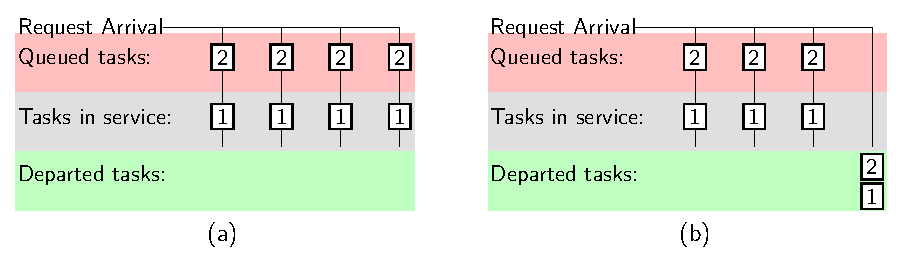
\includegraphics{MDS42}
%   \end{center}
%   \caption{Two possible $MDS(n,2)$ system scenarios: (a) all tasks start being served simultaneously and (b) one of the tasks departs earlier than the remaining  $(n-1)$.}\label{fig:fig_mds_n_2_start_setup}
% \end{figure*}

% In the system shown in Fig.~\ref{fig:fig_mds_n_2_start_setup}, only two jobs are present in the system and all the tasks of the job $1$ starts simultaneously as in the complete-start setup as shown in part $(a)$. When a single task of job $1$ departs, job $2$ enters the service in partial-start. Modeling the MDS setup as an M/G/1 queue where jobs arrive and depart in order, PK formula gives the average system time for an arbitrary job as follows:
% \[ E[T_{(n,2)}] = E[V_{(n,2)}] + \frac{\lambda E[V_{(n,2)}^2]}{2(1 - \lambda E[V_{(n,2)}])} \]
% where the first ($E[V_{(n,2)}]$) and the second ($E[V_{(n,2)}^2]$) moments of the job service time can be computed as
% \begin{equation}
%   \label{eq:eq_mds_n_2_serv_time_moments}
%   \begin{split}
%     & E[V_{(n,2)}] = f_J(p)E[V_p] + f_J(c)E[V_c] \\
%     & E[V_{(n,2)}^2] = f_J(p)E[V_p^2] + f_J(c)E[V_c^2]
%   \end{split}
% \end{equation}

% Consider the homogeneous case where all the servers have identical exponential service time with rate $\mu$. In the partial-start, completion of any one of the $n-1$ tasks that started service simultaneously signals the job termination, so $V_p$ is $Exp((n-1)\mu)$ where $E[V_p] = ((n-1)\mu)^{-1}$, $E[V_p^2] = 2((n-1)\mu)^{-2}$. In the complete-start, job is completed with the first two task completions, so using the order statistics $E[V_c] = (H_n - H_{n-2})\mu^{-1}$ where $H_n = \sum_{k=1}^{n} 1/k$ and $E[V_c^2] = (H_{n^2} - H_{(n-2)^2})\mu^{-2} + E[V_c]^2$ where $H_{n^2} = \sum_{k=1}^{n} 1/k^2$. We still need the values for $f_J(p)$ and $f_J(c)$ for \eqref{eq:eq_mds_n_2_serv_time_moments}.

% We next observe that only one server at a time can be ahead with task execution, and thus, there is at most one server whose queue is shorter while all others have the same queue size. To define the state of the system, we use the join queue where the departing tasks wait for their siblings to finish service. We define the state of the join queue to be the number of tasks $n(t)$ waiting for their siblings at time $t$. Only the tasks that departed from the same server can be in the join queue simultaneously and the server with the shortest queue cannot be labeled anyhow since the servers are identical. In addition, by using the number of jobs $N(t)$ that are waiting or in service in the servers at time $t$, we observe that the state of the overall system $(N(t), n(t))$ is Markov, which is drawn in Fig.~\ref{fig:fig_mds_n_2_mp_full__high_traff} together with the simplified version by the high-traffic assumption.
% \begin{figure}[htb]
%   \begin{center}
%     \begin{tikzpicture}  
%       \node at (0,3) {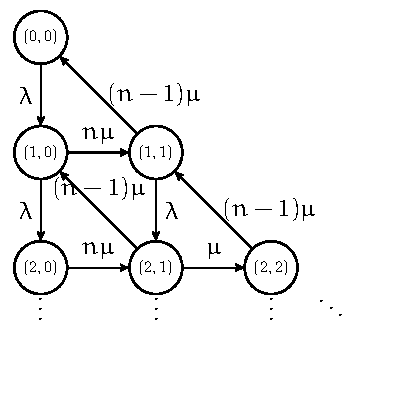
\includegraphics{MDSn2}};
%       \node at (0,0)  { 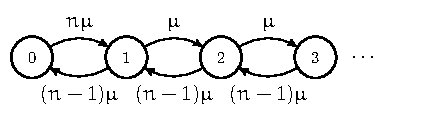
\includegraphics{MDSn2JoinHighT}};
%     \end{tikzpicture}
%   \end{center}
%   \vspace*{-0.5cm}
%   \caption{Markov process (a) for the MDS(n,2) and (b) its high-traffic approximation.}
%   \label{fig:fig_mds_n_2_mp_full__high_traff}
% \end{figure}

% % High-traffic discussion
% Repeating the assumption of "high-traffic regime" here, suppose $\lambda$ is very close to its critical value and the queues are never empty. The state of the join queue $n(t)$ itself is a simple Markov process shown in Fig.~\ref{fig:fig_mds_n_2_mp_full__high_traff}(b). Markov process for the high traffic regime can be obtained from the one in Fig.~\ref{fig:fig_mds_n_2_mp_full__high_traff}(a) as follows: (1) Introduce artificial transitions of rate $n\mu$ from state $(0,0)$ to $(1,1)$ and transitions of rate $\mu$ from state $(i,i)$ to $(i+1,i+1)$ for $i \geq 1$, (2) Gather all the states $(i,j)$ for all $i \geq 0$ into a "super-state", (3) Observe that process represented with these super-states is the same as the process for high-traffic regime. Thus, average job system time under high-traffic regime will give a lower bound on the average system time by a job under stable working conditions. Steady-state balance equations for the process under high-traffic regime is shown in \eqref{eq:eq_mds_n_2_join_balance_high_traffic}.
% \begin{equation}
%   \label{eq:eq_mds_n_2_join_balance_high_traffic}
%   n\mu p_0 = (n-1)\mu p_1 \quad\text{and}\quad \mu p_i = (n-1)
% \end{equation}
% where $lim_{t \rightarrow \infty} Pr\{n(t) = i\} = p_i$. Solving balance equations:
% \begin{equation}
%   \label{eq:eq_mds_n_2_steady_state}
%   p_i = (\frac{1}{n-1})^i n p_0, \quad i \geq 1, \quad\text{and}\quad p_0 = \frac{1}{1 + \frac{n}{n-2}}.
% \end{equation}
% from which $p_i$ can be computed. Since total transition rate of leaving the state is same for each state, steady-state probabilities $\pi_i$ for the states in the embedded Markov chain is same with the ones for $n(t)$.

% Under high-traffic regime, there is always a job in the queue waiting to receive service. Thus using the same argument that we used for the simplex setup, every transition in the Markov chain embedded in $n(t)$ that is triggered by a departing job defines the starting setup of the subsequent job and limiting fraction of the jobs that make partial ($f_{jp}$) or complete-start ($f_{jc}$) can be found as following. Let $f_{jd}$ represent the fraction of transitions corresponding to all the job departures and let $f_c$ represent the fraction of transitions into a complete-start setup for the subsequent job. Then, the values of $f_{jp}$ and $f_{jc}$ can be calculated as
% \begin{align*}
%  & f_{jd} = \sum_{i=1}^{\infty} \frac{n-1}{n}\pi_i = \frac{n-1}{n}(1-\pi_0), \\
%  & f_c = \frac{n-1}{n}\pi_1 = \frac{n-1}{n}\frac{n}{n-1} \pi_0 = \pi_0, \\
%  & f_{jc} = \frac{f_c}{f_{jd}} = \frac{n\pi_0}{(n-1)(1-\pi_0)} \quad\text{and}\quad f_{jp} = 1 - f_{jc}
% \end{align*}
% Note that $f_{jc}$ serves as a lower bound on $f_J(c)$ and consequently $f_{jp}$ serves as an upper bound on $f_J(p)$ because of the high-traffic regime assumption. Plugging $f_{jc}$ and $f_{jp}$ for $f_J(c)$ and $f_J(p)$ respectively in \eqref{eq:eq_mds_n_2_serv_time_moments} will give the values for $E[V_{(n,2)}]$, $E[V_{(n,2)}^2]$, and finally $E[T_{(n,2)}]$ which is a lower bound as discussed. Fig.~\ref{fig:fig_mds_n_2_E_T_sim_model_comparison} shows that discussed M/G/1 model serves as a lower bound for the MDS(n,2) which performs better than the lower bound presented in \cite{joshi2012coding}, however it performs slightly worse for low arrival rates. As also expected, as the arrival rate $\lambda$ increases, the model becomes more and more accurate since the system starts to experience the assumed high-traffic load.
% \begin{figure*}[h]
%  \centering
%  \begin{tabular}{cc}
% %    \subfloat[]{\includegraphics[width=0.45\textwidth, keepaspectratio=true]{fig_mds_3_2_E_T_sim_model_comparison.png} }
% %    \subfloat[]{\includegraphics[width=0.45\textwidth, keepaspectratio=true]{fig_mds_4_2_E_T_sim_model_comparison.png} } \\
% %    \subfloat[]{\includegraphics[width=0.45\textwidth, keepaspectratio=true]{fig_mds_5_2_E_T_sim_model_comparison.png} }
% %    \subfloat[]{\includegraphics[width=0.45\textwidth, keepaspectratio=true]{fig_mds_6_2_E_T_sim_model_comparison.png} } \\
%   \begin{subfigure}[h]{.45\textwidth}
%     \centering
%     \includegraphics[width=1\textwidth, keepaspectratio=true]{fig_mds_3_2_E_T_sim_model_comparison.png}
%   \end{subfigure}
%   \begin{subfigure}[h]{.45\textwidth}
%     \centering
%     \includegraphics[width=1\textwidth, keepaspectratio=true]{fig_mds_4_2_E_T_sim_model_comparison.png}
%   \end{subfigure}
%   \begin{subfigure}[h]{.45\textwidth}
%     \centering
%     \includegraphics[width=1\textwidth, keepaspectratio=true]{fig_mds_5_2_E_T_sim_model_comparison.png}
%   \end{subfigure}
%   \begin{subfigure}[h]{.45\textwidth}
%     \centering
%     \includegraphics[width=1\textwidth, keepaspectratio=true]{fig_mds_6_2_E_T_sim_model_comparison.png}
%   \end{subfigure}
%  \end{tabular}
%  \caption{Simulation results showing the upper and lower bounds, modeled and the simulated average system time for MDS(n,2). Upper bound (shown with legend sm\_mds\_*) is obtained by the split-merge model discussed in \cite{joshi2012coding} and the lower bound (shown with legend varki\_mds\_*) is presented in \cite{joshi2012coding}.}
%  \label{fig:fig_mds_n_2_E_T_sim_model_comparison}
% \end{figure*}

%%%%%%%%%%%%%%%%%%%%%%%%%%%%%%%%%%%%%%%%%%%%%%%%%%%%%%%%%%%%%%%%%%%%%%%%%%%%%%%%
% \bibliographystyle{IEEEtran}
\bibliographystyle{ACM-Reference-Format}
\bibliography{references}
\end{document}